\documentclass[12pt, letterpaper]{article}

\usepackage[margin=1in]{geometry}
\usepackage{amsmath, amssymb}
\usepackage{graphicx}
\usepackage{booktabs}
\usepackage{hyperref}
\usepackage{natbib}
\usepackage{xcolor}
\usepackage{caption}
\usepackage{subcaption}

\hypersetup{
    colorlinks=true,
    linkcolor=blue!60!black,
    citecolor=blue!60!black,
    urlcolor=blue!60!black,
}

\newcommand{\Msun}{M_\odot}
\newcommand{\Mh}{M_\mathrm{h}}
\newcommand{\Mstar}{M_*}
\newcommand{\DS}{\Delta\Sigma}
\newcommand{\beff}{b_\mathrm{eff}}
\newcommand{\ngal}{n_\mathrm{gal}}
\newcommand{\seff}{\sigma_\mathrm{eff}}
\newcommand{\sobs}{\sigma_\mathrm{obs}}
\newcommand{\sSHMR}{\sigma_\mathrm{SHMR}}

\title{Fisher Forecast for the Stellar--Halo Mass Relation\\
in the Dwarf Galaxy Regime with Spec-S5}
\author{SHMR Fisher Forecast Pipeline}
\date{March 2026}

\begin{document}
\maketitle

\begin{abstract}
We present a Fisher matrix forecast assessing how well current and
next-generation spectroscopic surveys, combined with Stage-IV imaging
weak lensing, can constrain the stellar--halo mass relation (SHMR) in
the dwarf galaxy regime ($\Mstar < 10^{9}\,\Msun$).
Four survey scenarios spanning DESI through a futuristic Stage-V
``Dwarf Mania'' concept are compared in two configurations: a
dwarf-only forecast ($\log\Mstar \in [7, 9]$) and a full stellar mass
range forecast ($\log\Mstar \in [7, 12]$).
We find that the low-mass slope $\beta_0$ and normalization $N_0$ of
the SHMR can be constrained to sub-percent precision by Spec-S5 and
Stage-V surveys, while the mass-dependent scatter parameters
($\sigma_\mathrm{high}$, $\sigma_\mathrm{rise}$) remain poorly
constrained ($>300\%$ fractional error) unless the sample spans the
full stellar mass range across both sides of the SHMR peak at
$\Mh \sim 10^{12}\,\Msun$.
With full-range coverage, scatter constraints improve by
$\sim\!100\times$, reaching $\sim\!1\%$ precision on
$\sigma_\mathrm{high}$ for Stage-V.
\end{abstract}

\tableofcontents
\newpage

%% ================================================================
\section{Executive Summary}
\label{sec:executive}

\subsection{Science Motivation}

The stellar--halo mass relation (SHMR) is the central empirical
mapping between dark matter halos and the galaxies they host.
While the SHMR is well-constrained around $\Mh \sim 10^{12}\,\Msun$
(the Milky Way regime), the dwarf galaxy regime ($\Mstar < 10^{9.5}\,
\Msun$, $\Mh < 10^{11.5}\,\Msun$) remains poorly characterized due
to the difficulty of obtaining spectroscopic redshifts for faint,
low-surface-brightness galaxies.
Spec-S5 and other next-generation spectroscopic surveys will
dramatically increase the number of dwarf galaxies with
spectroscopic redshifts, enabling precise galaxy--galaxy lensing and
clustering measurements that directly probe the SHMR at low masses.

\subsection{Forecast Pipeline Overview}

The forecast pipeline computes the Fisher information matrix from
three observables per (redshift, stellar mass) bin:
\begin{enumerate}
    \item \textbf{Galaxy--galaxy lensing} $\DS(R)$: the excess surface
    mass density around lens galaxies, computed from an HOD-weighted
    NFW 1-halo profile plus an analytic linear-bias 2-halo term.
    \item \textbf{Effective bias} $\beff$: the HOD-weighted mean
    linear halo bias, probing halo mass through large-scale clustering.
    \item \textbf{Stellar mass function} $\Phi$: the galaxy number
    density per stellar mass bin, with a covariance model that includes
    both Poisson noise and cosmic variance.
\end{enumerate}

Key pipeline features:
\begin{itemize}
    \item \textbf{SHMR model:} Moster et al.\ (2013) double
    power-law with linear $z/(1+z)$ evolution (8 shape parameters).
    \item \textbf{Mass-dependent scatter:} Cao \& Tinker (2020)
    $\tanh$ parameterization with $\sigma(\Mh)$ varying from $0.18$
    dex at high $\Mh$ to $0.38$ dex at low $\Mh$.
    \item \textbf{Stellar mass uncertainty:}
    $\sobs = 0.1$ dex for spectroscopic surveys, incorporated as
    $\seff = \sqrt{\sSHMR^2 + \sobs^2}$.
    \item \textbf{Nuisance parameters:} multiplicative shear
    calibration bias ($\sigma_m = 0.02$) and source photo-$z$ bias
    ($\sigma_{\delta z} = 0.03$), marginalized with Gaussian priors.
    \item \textbf{Systematic floor:} 5\% irreducible systematic
    uncertainty on $\DS$ from baryonic effects, miscentering, and
    photometric calibration.
    \item \textbf{Fixed imaging survey:} Stage-IV lensing
    ($n_\mathrm{source} = 25\,\mathrm{arcmin}^{-2}$,
    $\sigma_e = 0.26$, $z_\mathrm{source,med} = 1.0$).
\end{itemize}

\subsection{Key Conclusions}

\begin{enumerate}
    \item \textbf{Shape parameters are well-constrained by dwarfs
    alone.}
    Even the most limited survey (DESI, $10^5$ galaxies) constrains
    the low-mass slope $\beta_0$ to $3.3\%$ and the normalization
    $N_0$ to $17\%$.
    Spec-S5 ($10^7$ galaxies, $\log\Mstar_\mathrm{min} = 7.0$)
    achieves sub-percent precision on $\beta_0$ ($1.0\%$) and $4.4\%$
    on $N_0$.

    \item \textbf{Scatter constraints require the full stellar mass
    range.}
    In the dwarf-only configuration, even the Stage-V survey cannot
    constrain $\sigma_\mathrm{high}$ or $\sigma_\mathrm{rise}$ to
    better than $\sim\!300\%$ fractional error.
    This is because all dwarf halos sit on the same side of the SHMR
    peak, where scatter primarily smears galaxies within the same
    regime without creating distinctive signatures across multiple
    bins.

    \item \textbf{Full-range coverage transforms scatter constraints.}
    Extending to $\log\Mstar \in [7, 12]$ enables $\sim\!100\times$
    improvement in scatter precision, reaching $0.9\%$ on
    $\sigma_\mathrm{high}$ and $3.6\%$ on $\sigma_\mathrm{rise}$ for
    Stage-V.
    The critical lever arm comes from spanning both sides of the SHMR
    peak at $\Mh \sim 10^{12}\,\Msun$.

    \item \textbf{Spec-S5 delivers 3--6$\times$ improvement over DESI}
    across all SHMR parameters in the dwarf regime, driven by deeper
    stellar mass completeness ($\log\Mstar_\mathrm{min} = 7.0$ vs.\
    $8.0$) and larger galaxy samples.
\end{enumerate}


%% ================================================================
\section{Survey Configurations}
\label{sec:surveys}

We compare four spectroscopic survey scenarios, all combined with the
same Stage-IV imaging weak lensing survey.
Two forecast configurations are run for each survey:
(i) a \emph{dwarf-only} configuration restricted to
$\log\Mstar < 9.0$ with the high-mass SHMR parameters
($\gamma_0$, $\log M_{1,0}$) fixed, and
(ii) a \emph{full-range} configuration spanning $\log\Mstar \in [7, 12]$
with all SHMR shape and scatter parameters freed and galaxy counts
scaled by $3\times$ to reflect the larger samples available when the
full stellar mass range is included.

\subsection{Dwarf-Only Configuration}

\begin{table}[htbp]
\centering
\caption{Survey parameters for the dwarf-only forecast. All surveys
use $\Delta\log\Mstar = 0.5\,\mathrm{dex}$ bins and fix
$\gamma_0 = 0.608$ and $\log M_{1,0} = 11.59$. The varied SHMR
parameters are $N_0$, $\beta_0$, $\sigma_\mathrm{high}$,
$\sigma_\mathrm{rise}$, plus two nuisance parameters (shear
calibration $m$ and source photo-$z$ bias $\delta z_s$).}
\label{tab:surveys_dwarf}
\begin{tabular}{lcccccc}
\toprule
Survey & Area & $z$-range & $N_\mathrm{gal}$ &
$\log\Mstar_\mathrm{min}$ & $\log\Mstar_\mathrm{max}$ &
$N_\mathrm{M*\text{-bins}}$ \\
 & [deg$^2$] & & & [dex] & [dex] & \\
\midrule
DESI         & 14\,000 & 0.01--0.08 & $10^5$     & 8.0 & 9.0 & 2 \\
DESI-II      &  5\,000 & 0.01--0.15 & $10^6$     & 7.5 & 9.0 & 3 \\
Spec-S5      &  5\,000 & 0.01--0.20 & $1.2\times10^7$ & 7.0 & 9.0 & 4 \\
Stage-V DM   &  8\,000 & 0.01--0.30 & $4\times10^7$   & 7.0 & 9.0 & 4 \\
\bottomrule
\end{tabular}
\end{table}

\subsection{Full Stellar Mass Range Configuration}

\begin{table}[htbp]
\centering
\caption{Survey parameters for the full-range forecast. The upper
stellar mass limit is extended to $\log\Mstar = 12.0$, and galaxy
counts are scaled by $3\times$ relative to the dwarf-only
configuration. All six $z=0$ SHMR shape parameters are varied:
$\log M_{1,0}$, $N_0$, $\beta_0$, $\gamma_0$, plus
$\sigma_\mathrm{high}$ and $\sigma_\mathrm{rise}$.}
\label{tab:surveys_fullrange}
\begin{tabular}{lcccccc}
\toprule
Survey & Area & $z$-range & $N_\mathrm{gal}$ &
$\log\Mstar_\mathrm{min}$ & $\log\Mstar_\mathrm{max}$ &
$N_\mathrm{M*\text{-bins}}$ \\
 & [deg$^2$] & & & [dex] & [dex] & \\
\midrule
DESI         & 14\,000 & 0.01--0.08 & $3\times10^5$     & 8.0 & 12.0 & 8 \\
DESI-II      &  5\,000 & 0.01--0.15 & $3\times10^6$     & 7.5 & 12.0 & 9 \\
Spec-S5      &  5\,000 & 0.01--0.20 & $3.6\times10^7$   & 7.0 & 12.0 & 10 \\
Stage-V DM   &  8\,000 & 0.01--0.30 & $1.2\times10^8$   & 7.0 & 12.0 & 10 \\
\bottomrule
\end{tabular}
\end{table}


%% ================================================================
\section{Forecast Results: Dwarf-Only}
\label{sec:results_dwarf}

\subsection{Lensing Signal and Signal-to-Noise}

Figure~\ref{fig:dwarf_ds} shows the predicted galaxy--galaxy lensing
signal $\DS(R)$ for the lowest common stellar mass bin
($\log\Mstar \in [8.0, 8.5]$ at $z = 0.05$), with $1\sigma$ error
bars for each survey.
The signal peaks at $\sim\!3\,\Msun/\mathrm{pc}^2$ near
$R \sim 0.05\,\mathrm{Mpc}$ and transitions from the 1-halo NFW
regime to the 2-halo linear-bias regime at $R \sim 0.3\,\mathrm{Mpc}$.
DESI (blue) has the largest error bars due to its small galaxy count
($10^5$) and narrow redshift range, while Stage-V (red) achieves the
smallest errors from its combination of large area, deep completeness,
and extended redshift range.

\begin{figure}[htbp]
\centering
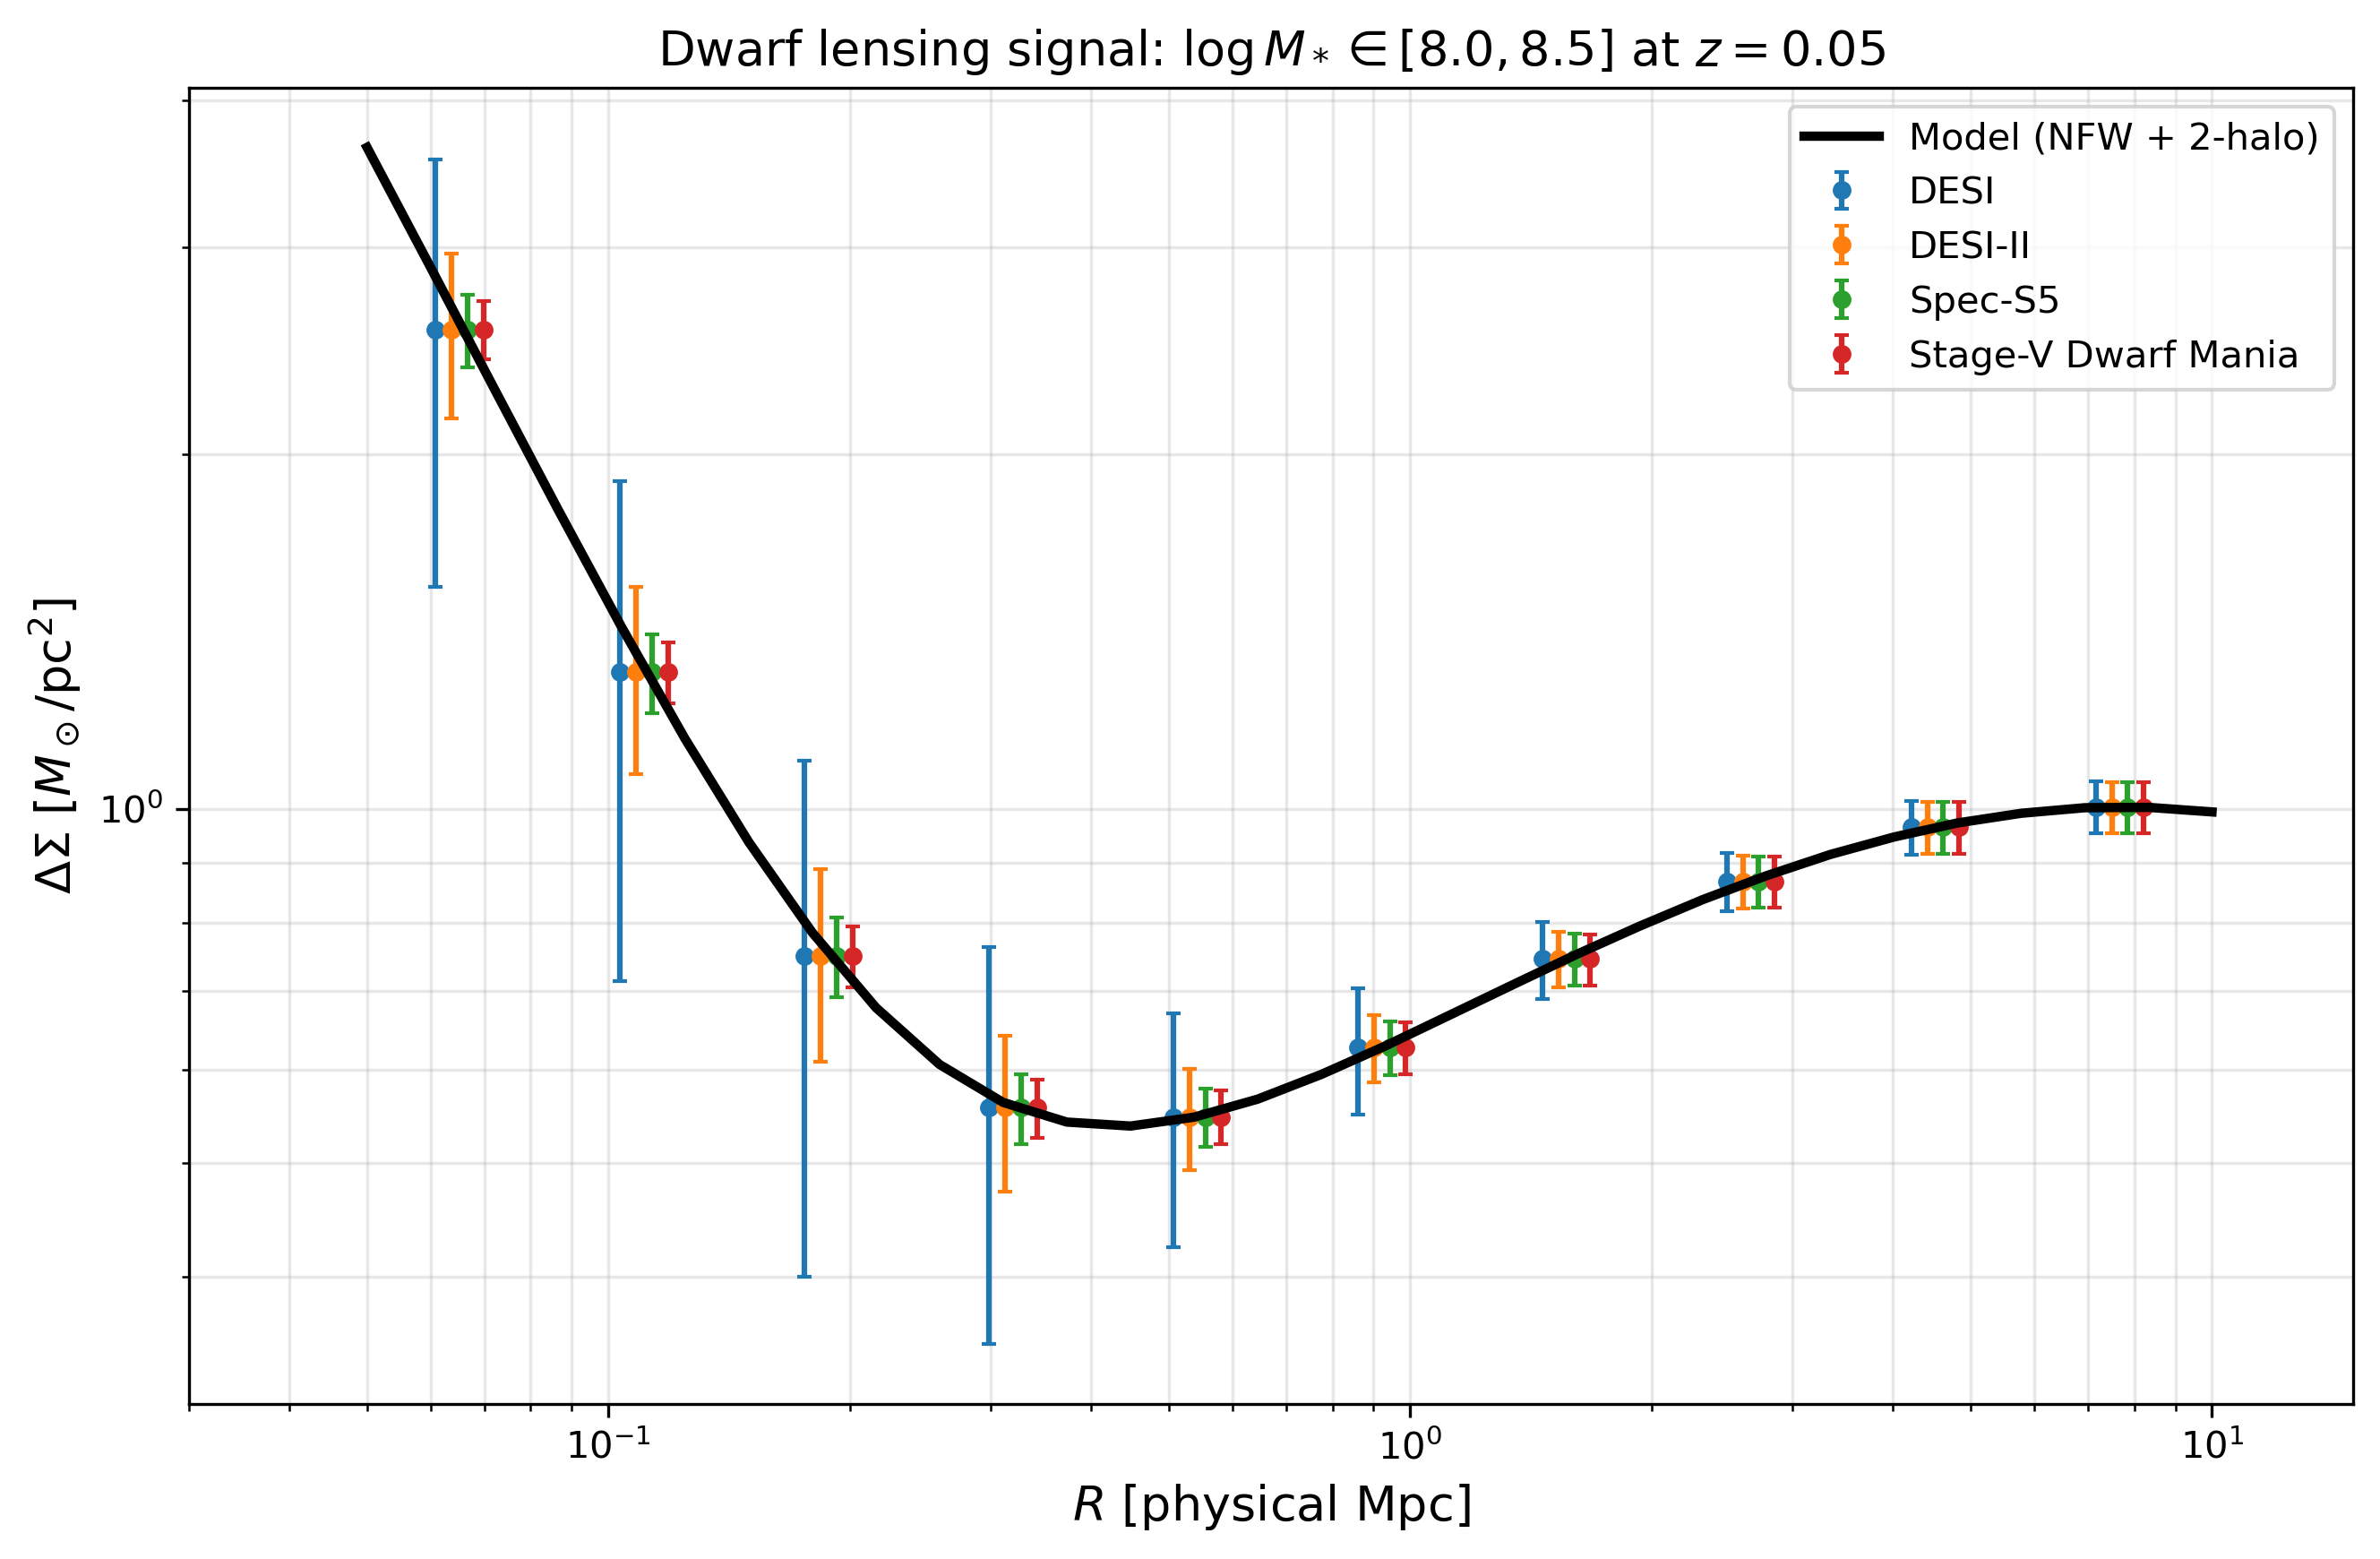
\includegraphics[width=0.85\textwidth]{figures/dwarf_delta_sigma.png}
\caption{Galaxy--galaxy lensing signal $\DS(R)$ in the dwarf stellar
mass bin $\log\Mstar \in [8.0, 8.5]$ at $z = 0.05$, with $1\sigma$
error bars for each survey. The solid black curve shows the model
prediction (NFW 1-halo + linear-bias 2-halo). Error bars include shape
noise from Stage-IV imaging lensing ($n_\mathrm{source} =
25\,\mathrm{arcmin}^{-2}$, $\sigma_e = 0.26$) plus a $5\%$ systematic
floor.  Radial bins span $R \in [0.01, 10]\,\mathrm{Mpc}$ with 30
log-spaced bins, emphasizing the 1-halo regime where most Fisher
information resides.}
\label{fig:dwarf_ds}
\end{figure}


\subsection{Parameter Constraints}

Figure~\ref{fig:dwarf_errors} presents the fractional parameter errors
$\sigma(\theta)/|\theta_\mathrm{fid}|$ for all four surveys.
The shape parameters ($N_0$, $\beta_0$) are well-constrained: Spec-S5
achieves $4.4\%$ on $N_0$ and $1.0\%$ on $\beta_0$, while Stage-V
reaches $3.1\%$ and $0.7\%$ respectively.
In contrast, the scatter parameters ($\sigma_\mathrm{high}$,
$\sigma_\mathrm{rise}$) have fractional errors exceeding $300\%$ for
all surveys, indicating that the dwarf-only sample cannot meaningfully
constrain the mass-dependent scatter model.

\begin{figure}[htbp]
\centering
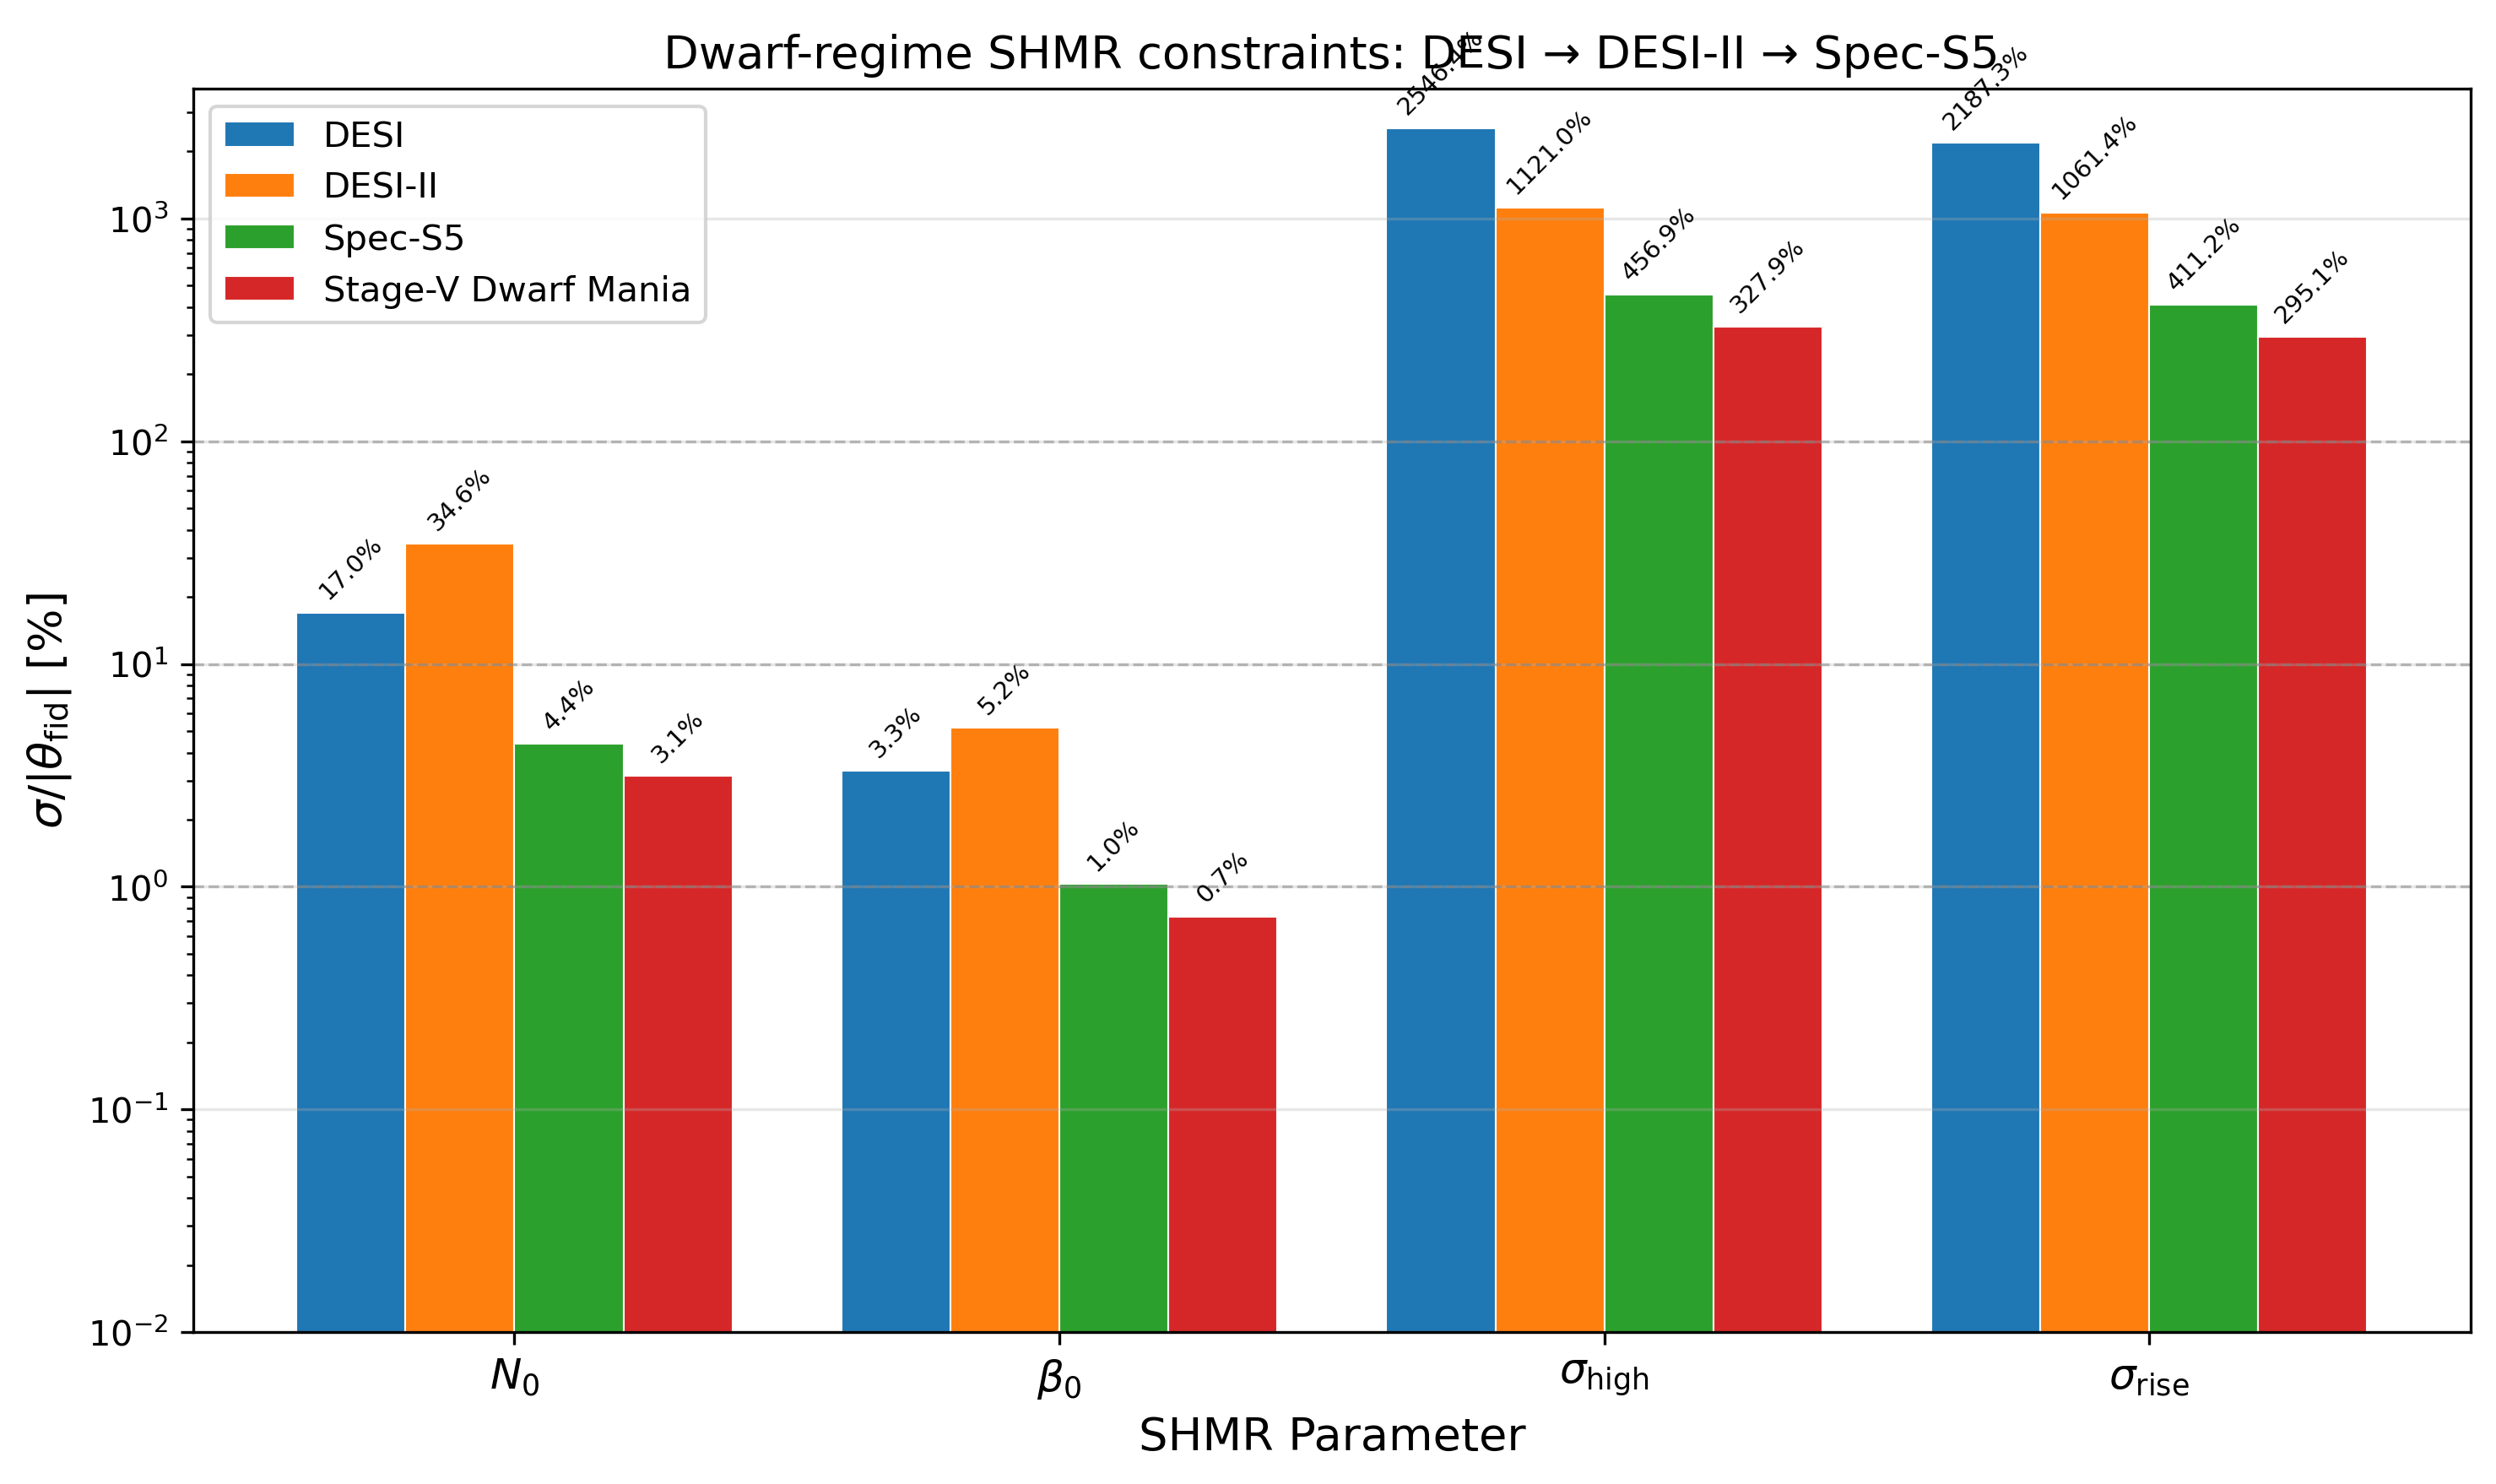
\includegraphics[width=0.85\textwidth]{figures/dwarf_error_comparison.png}
\caption{Fractional 1$\sigma$ parameter errors (log scale) for the
dwarf-only forecast. The SHMR shape parameters ($N_0$, $\beta_0$) are
constrained to a few percent, with systematic improvements from DESI
through Stage-V. The scatter parameters ($\sigma_\mathrm{high}$,
$\sigma_\mathrm{rise}$) remain unconstrained ($>300\%$) because all
dwarf halos probe the same side of the SHMR peak. Reference lines at
$1\%$, $10\%$, and $100\%$ are shown.}
\label{fig:dwarf_errors}
\end{figure}


\subsection{Fisher Ellipses and Parameter Degeneracies}

Figure~\ref{fig:dwarf_ellipses} shows the 2D Fisher forecast
ellipses (1$\sigma$ and 2$\sigma$) for three key parameter pairs.
The left panel ($N_0$ vs.\ $\beta_0$) shows compact, well-oriented
ellipses that tighten systematically from DESI to Stage-V.
The center panel ($\sigma_\mathrm{high}$ vs.\ $\sigma_\mathrm{rise}$)
reveals a tight degeneracy: the dwarf-only data constrains a
\emph{combination} of these parameters (the effective scatter at the
characteristic dwarf halo mass) but cannot disentangle the plateau
height from the transition steepness.
The right panel ($N_0$ vs.\ $\sigma_\mathrm{high}$) shows a mild
correlation between the SHMR normalization and the scatter amplitude.

\begin{figure}[htbp]
\centering
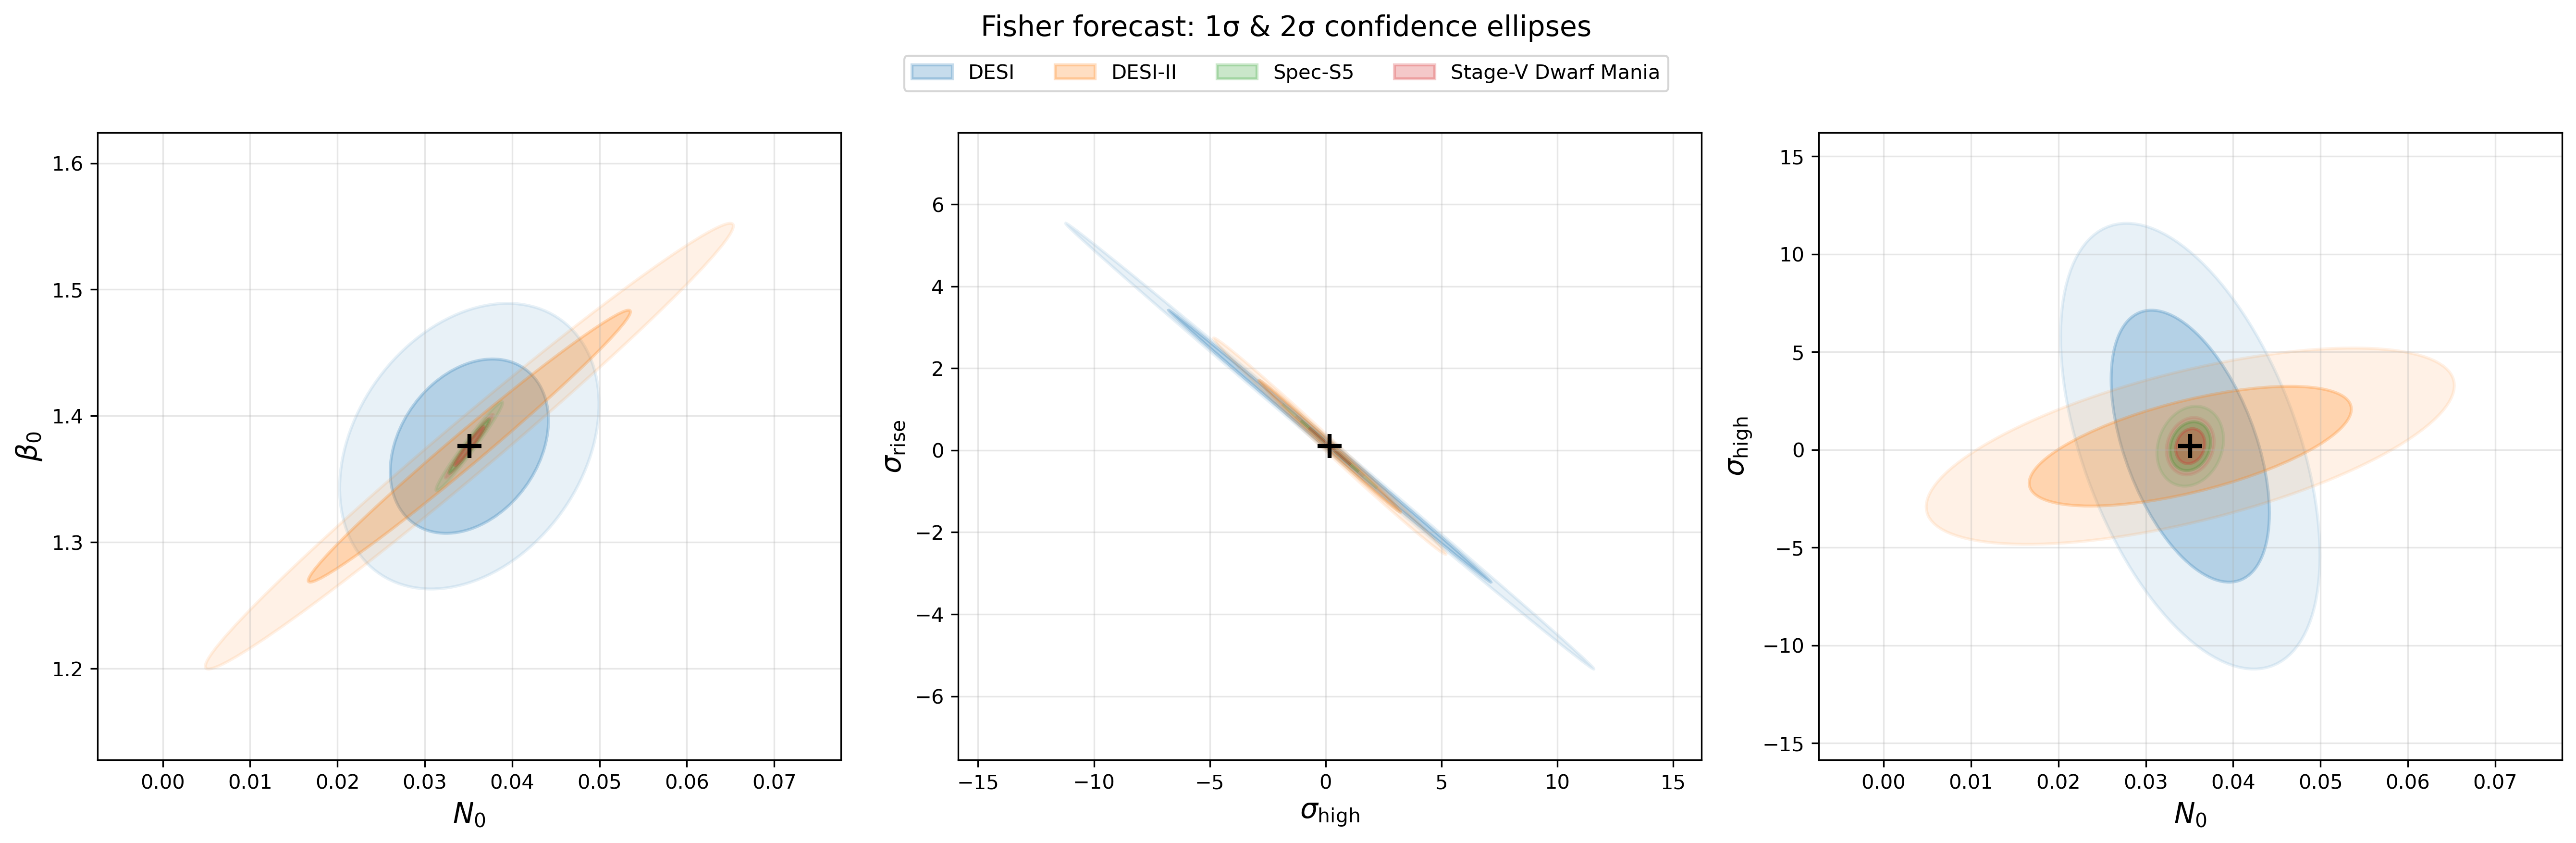
\includegraphics[width=\textwidth]{figures/dwarf_fisher_ellipses.png}
\caption{Fisher forecast 1$\sigma$ (dark shading) and 2$\sigma$ (light
shading) confidence ellipses for three parameter pairs in the
dwarf-only configuration. \textit{Left:} $N_0$ vs.\ $\beta_0$ ---
compact ellipses showing these shape parameters are well-constrained.
\textit{Center:} $\sigma_\mathrm{high}$ vs.\
$\sigma_\mathrm{rise}$ --- a strong degeneracy along a narrow axis
indicates that dwarf-only data constrains only a linear combination of
the scatter parameters. \textit{Right:} $N_0$ vs.\
$\sigma_\mathrm{high}$ --- mild correlation between normalization and
scatter. The fiducial parameter values are marked with a cross.}
\label{fig:dwarf_ellipses}
\end{figure}


\subsection{Relative Improvement over DESI}

Figure~\ref{fig:dwarf_improvement} quantifies the improvement factor
$\sigma(\mathrm{DESI})/\sigma(\mathrm{survey})$ for each survey
relative to DESI.
Spec-S5 achieves $3.2$--$5.6\times$ improvement across all parameters,
driven by its deeper stellar mass completeness
($\log\Mstar_\mathrm{min} = 7.0$ vs.\ $8.0$, adding two additional
low-mass bins) and $120\times$ more galaxies.
Stage-V provides a further factor of $\sim\!1.4$ beyond Spec-S5,
reaching $4.5$--$7.8\times$ improvement over DESI.
DESI-II is comparable to or slightly worse than DESI on shape
parameters (smaller area partially offsets the deeper sample), but
$\sim\!2\times$ better on scatter parameters due to the additional
low-mass bin at $\log\Mstar = 7.5$.

\begin{figure}[htbp]
\centering
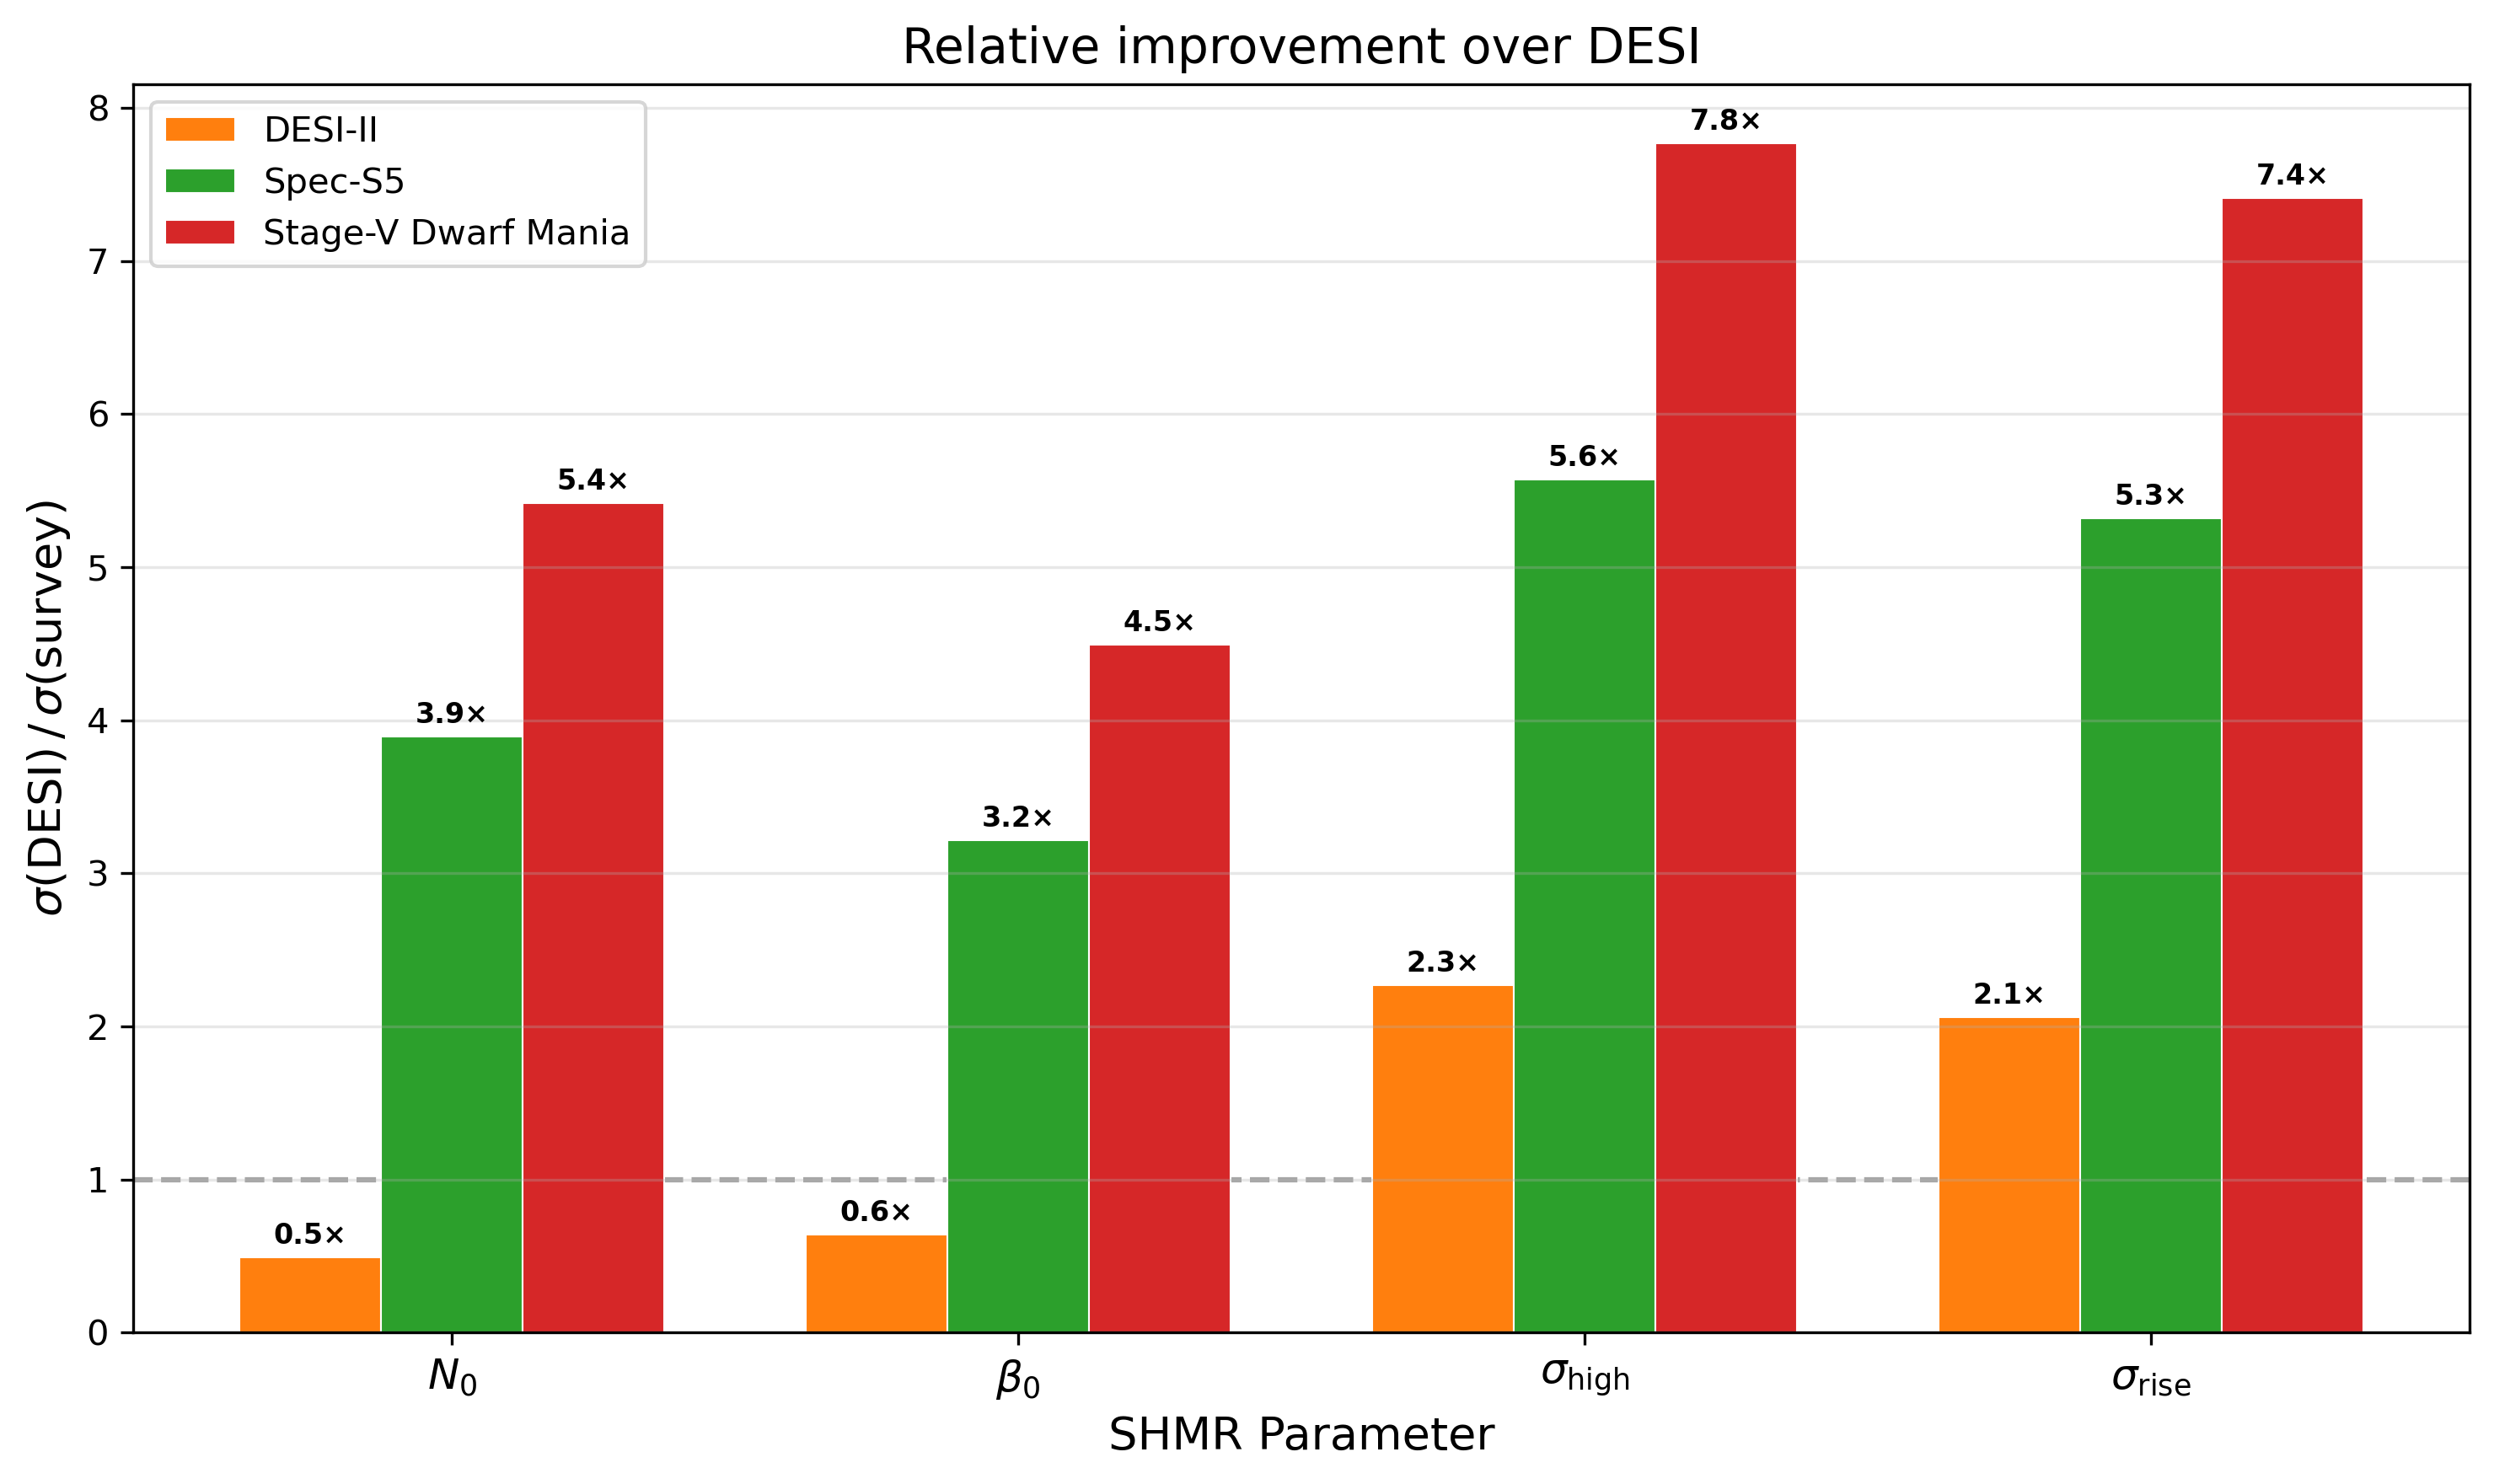
\includegraphics[width=0.85\textwidth]{figures/dwarf_relative_improvement.png}
\caption{Improvement factor
$\sigma(\mathrm{DESI})/\sigma(\mathrm{survey})$ for each SHMR
parameter relative to the DESI baseline. Values above 1 indicate
better constraints than DESI. Spec-S5 (green) achieves 3--6$\times$
improvement; Stage-V Dwarf Mania (red) reaches 4.5--8$\times$.
DESI-II (orange) is slightly worse than DESI on $N_0$ and $\beta_0$
due to its smaller area (5\,000 vs.\ 14\,000 deg$^2$) but better on
scatter parameters from the additional low-mass bin.}
\label{fig:dwarf_improvement}
\end{figure}


%% ================================================================
\section{Forecast Results: Full Stellar Mass Range}
\label{sec:results_fullrange}

Extending the stellar mass range to $\log\Mstar \in [7, 12]$
transforms the forecast by spanning both sides of the SHMR peak at
$\Mh \sim 10^{12}\,\Msun$.
With the full range, six SHMR shape parameters are varied
($\log M_{1,0}$, $N_0$, $\beta_0$, $\gamma_0$,
$\sigma_\mathrm{high}$, $\sigma_\mathrm{rise}$), and galaxy counts
are scaled by $3\times$.

\subsection{Parameter Constraints}

Figure~\ref{fig:fullrange_errors} shows fractional errors for the
full-range configuration.
All parameters are now constrained to $<12\%$ even for DESI; Stage-V
achieves sub-percent precision on all shape parameters and $0.9\%$ on
$\sigma_\mathrm{high}$.
The scatter parameter $\sigma_\mathrm{rise}$, which controls the
steepness of the scatter transition near $\Mh \sim 10^{12}\,\Msun$,
is constrained to $3.6\%$ by Stage-V (compared to $295\%$ in the
dwarf-only case --- a $\sim\!80\times$ improvement).

\begin{figure}[htbp]
\centering
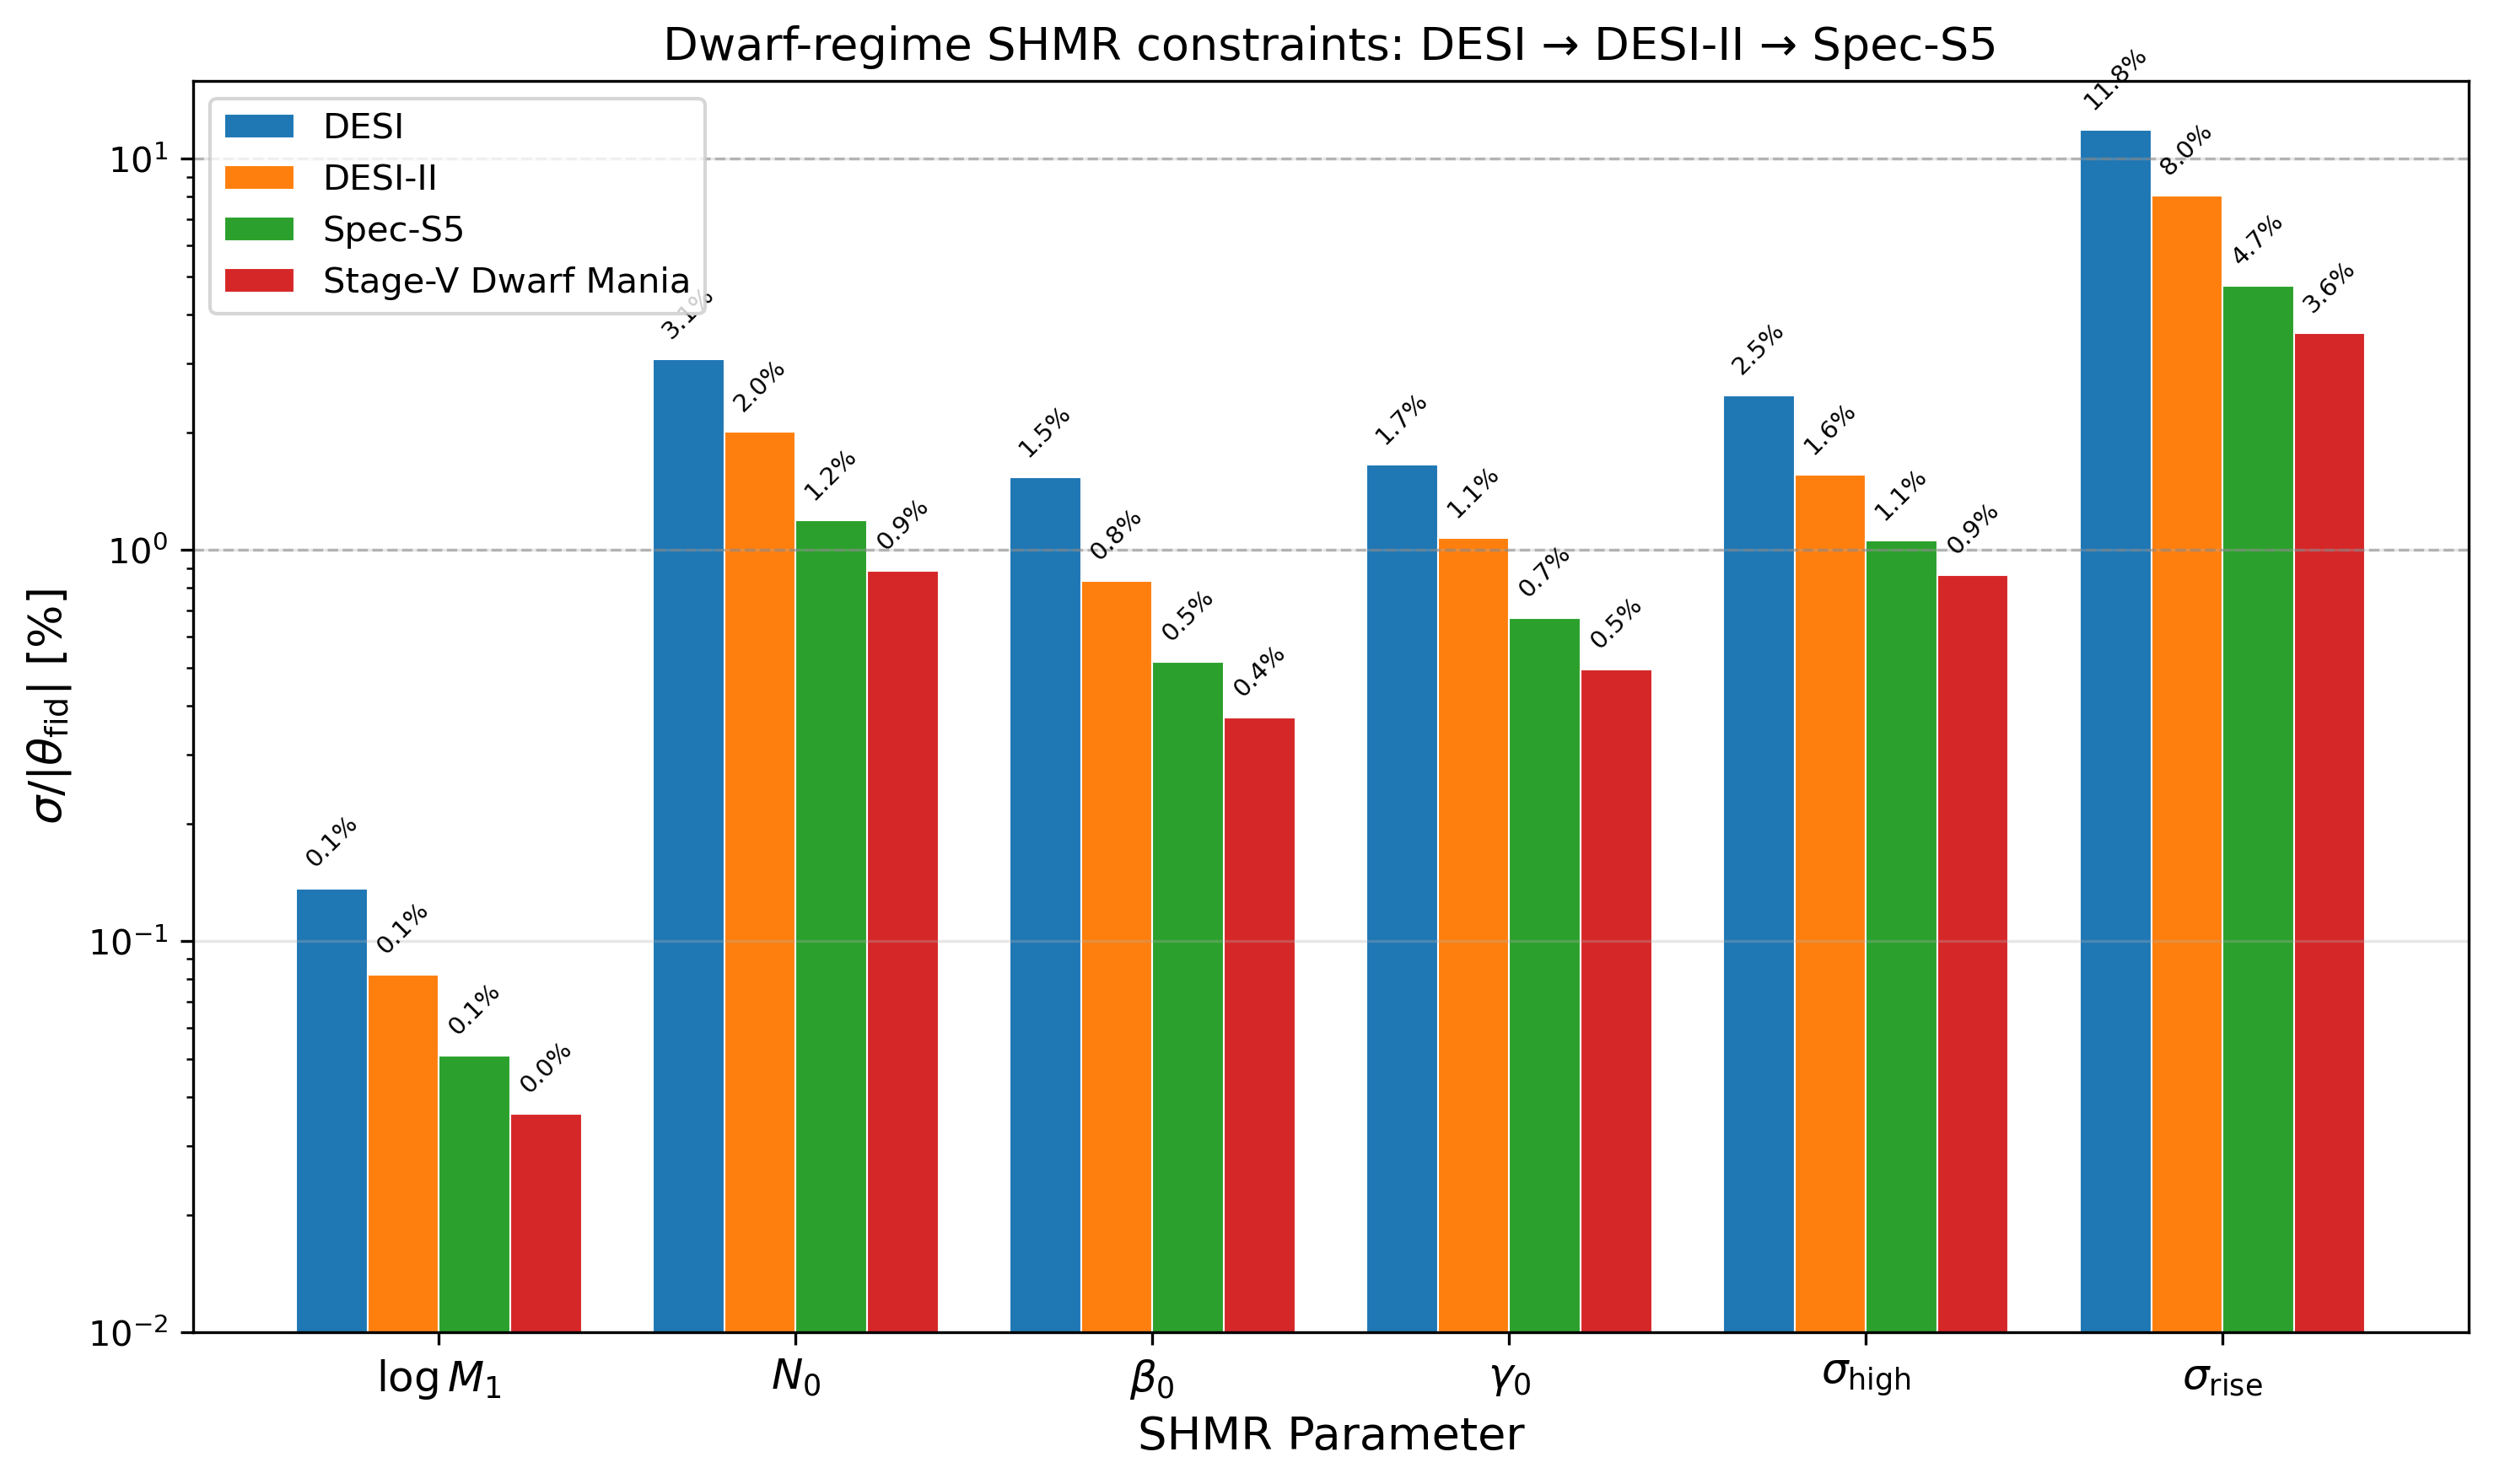
\includegraphics[width=0.85\textwidth]{figures/fullrange_error_comparison.png}
\caption{Fractional 1$\sigma$ errors for the full stellar mass range
forecast ($\log\Mstar \in [7, 12]$). All six SHMR parameters are now
well-constrained ($<12\%$). Stage-V reaches sub-percent precision on
all shape parameters, with $\sigma_\mathrm{high}$ constrained to
$0.9\%$ --- a $\sim\!360\times$ improvement over the dwarf-only
forecast.}
\label{fig:fullrange_errors}
\end{figure}


\subsection{Fisher Ellipses}

Figure~\ref{fig:fullrange_ellipses} shows the Fisher ellipses for the
full-range case.
The $\sigma_\mathrm{high}$--$\sigma_\mathrm{rise}$ degeneracy
(center panel) is dramatically reduced compared to the dwarf-only case
(Figure~\ref{fig:dwarf_ellipses}): the ellipses are compact rather
than razor-thin, indicating that the full mass range breaks the
degeneracy between the scatter plateau and transition steepness.
The physical mechanism is that high-mass bins ($\Mstar > 10^{10.5}$)
probe halos where $\sigma \to \sigma_\mathrm{high}$, while dwarf bins
probe halos where $\sigma \to \sigma_\mathrm{high} +
2\sigma_\mathrm{rise}$; together they separate the two parameters.

\begin{figure}[htbp]
\centering
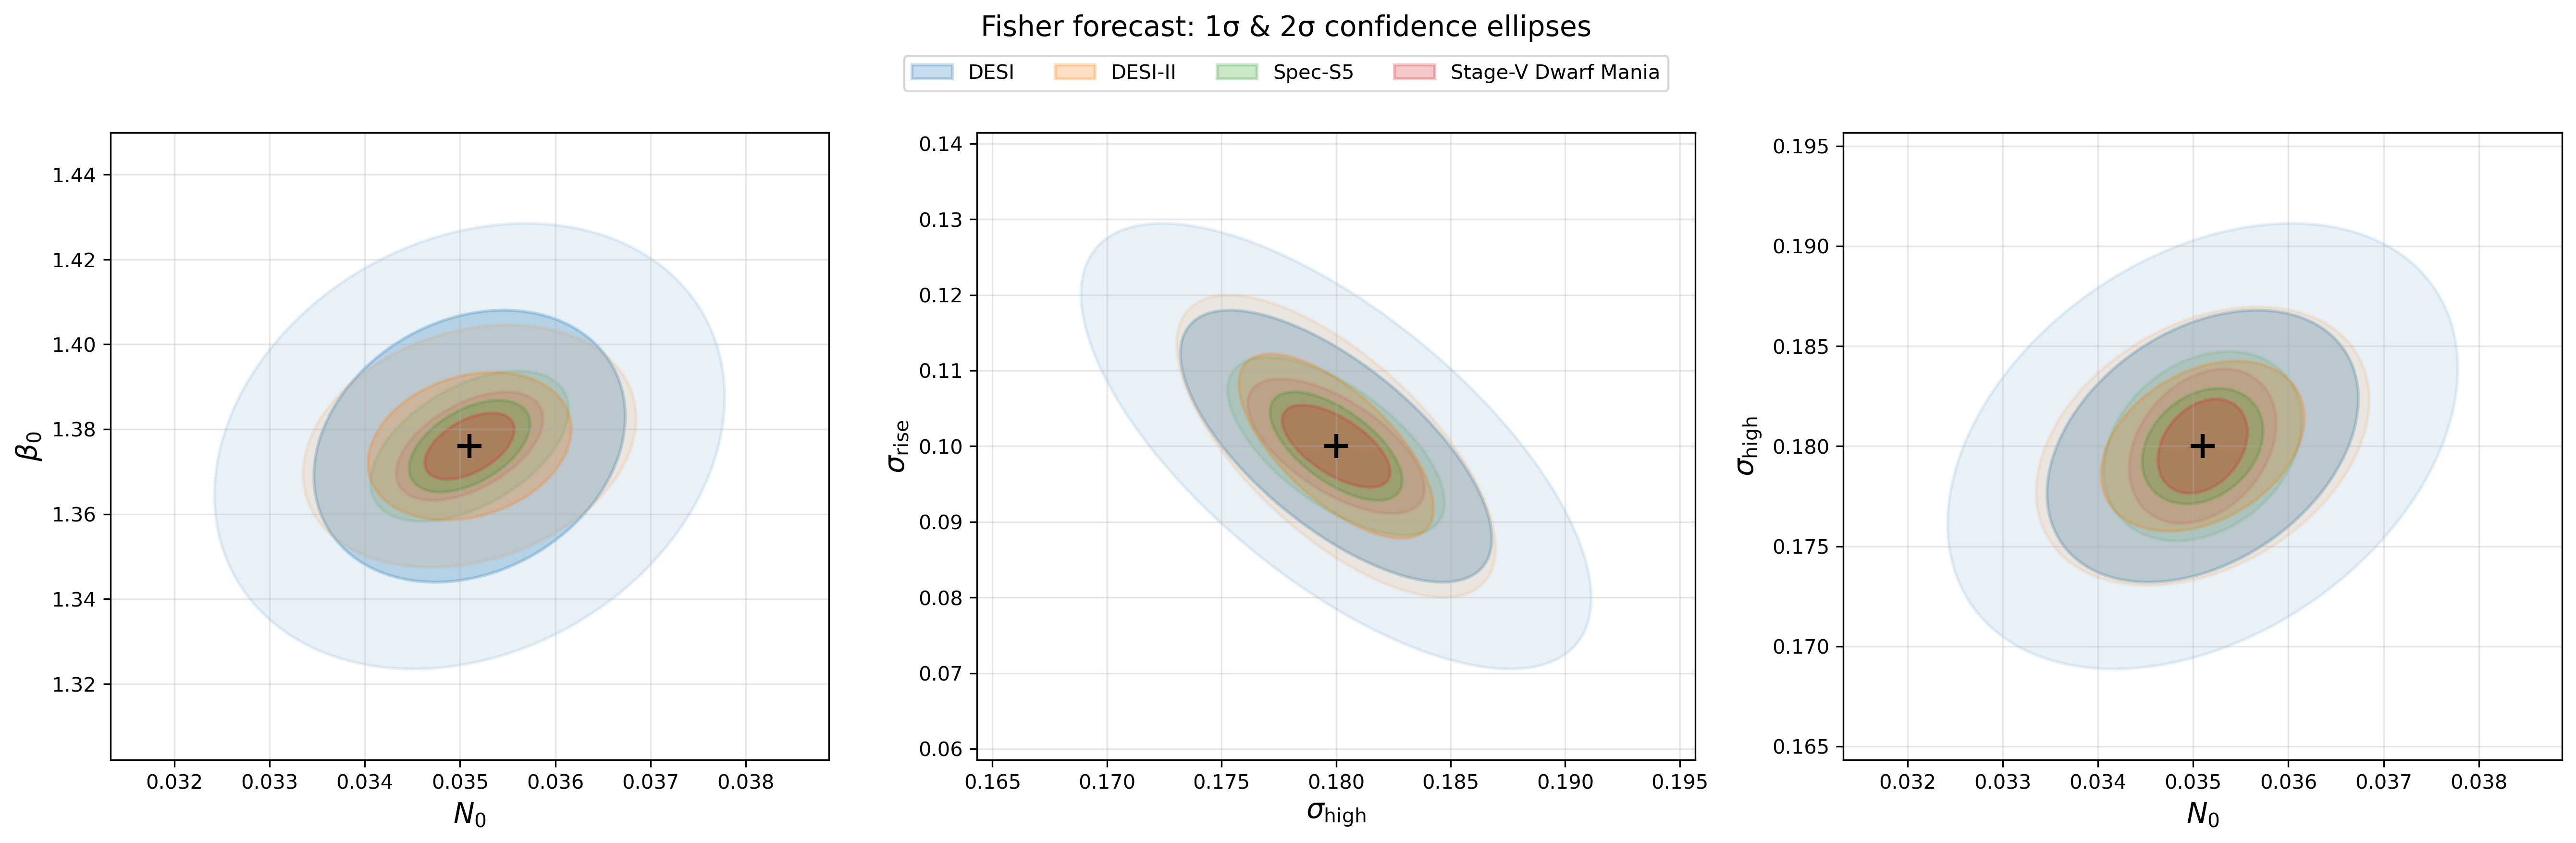
\includegraphics[width=\textwidth]{figures/fullrange_fisher_ellipses.png}
\caption{Fisher ellipses for the full stellar mass range forecast.
Compared to the dwarf-only case (Figure~\ref{fig:dwarf_ellipses}),
the $\sigma_\mathrm{high}$--$\sigma_\mathrm{rise}$ degeneracy
(center) is broken by spanning both sides of the SHMR peak. All
parameter pairs show compact, well-separated ellipses, with Stage-V
(innermost) achieving $\sim\!3\times$ tighter constraints than DESI
(outermost).}
\label{fig:fullrange_ellipses}
\end{figure}


\subsection{Relative Improvement}

Figure~\ref{fig:fullrange_improvement} shows the improvement factors
for the full-range case.
The gains are more uniform across parameters compared to the
dwarf-only case: Stage-V achieves $2.9$--$4.1\times$ improvement over
DESI on all six parameters, with the largest gain on $\beta_0$
($4.1\times$) driven by the low-mass bins that sensitively probe the
SHMR slope.
Spec-S5 achieves $2.4$--$3.0\times$ improvement, establishing it as
the primary science driver for constraining the SHMR at the
next-generation level.

\begin{figure}[htbp]
\centering
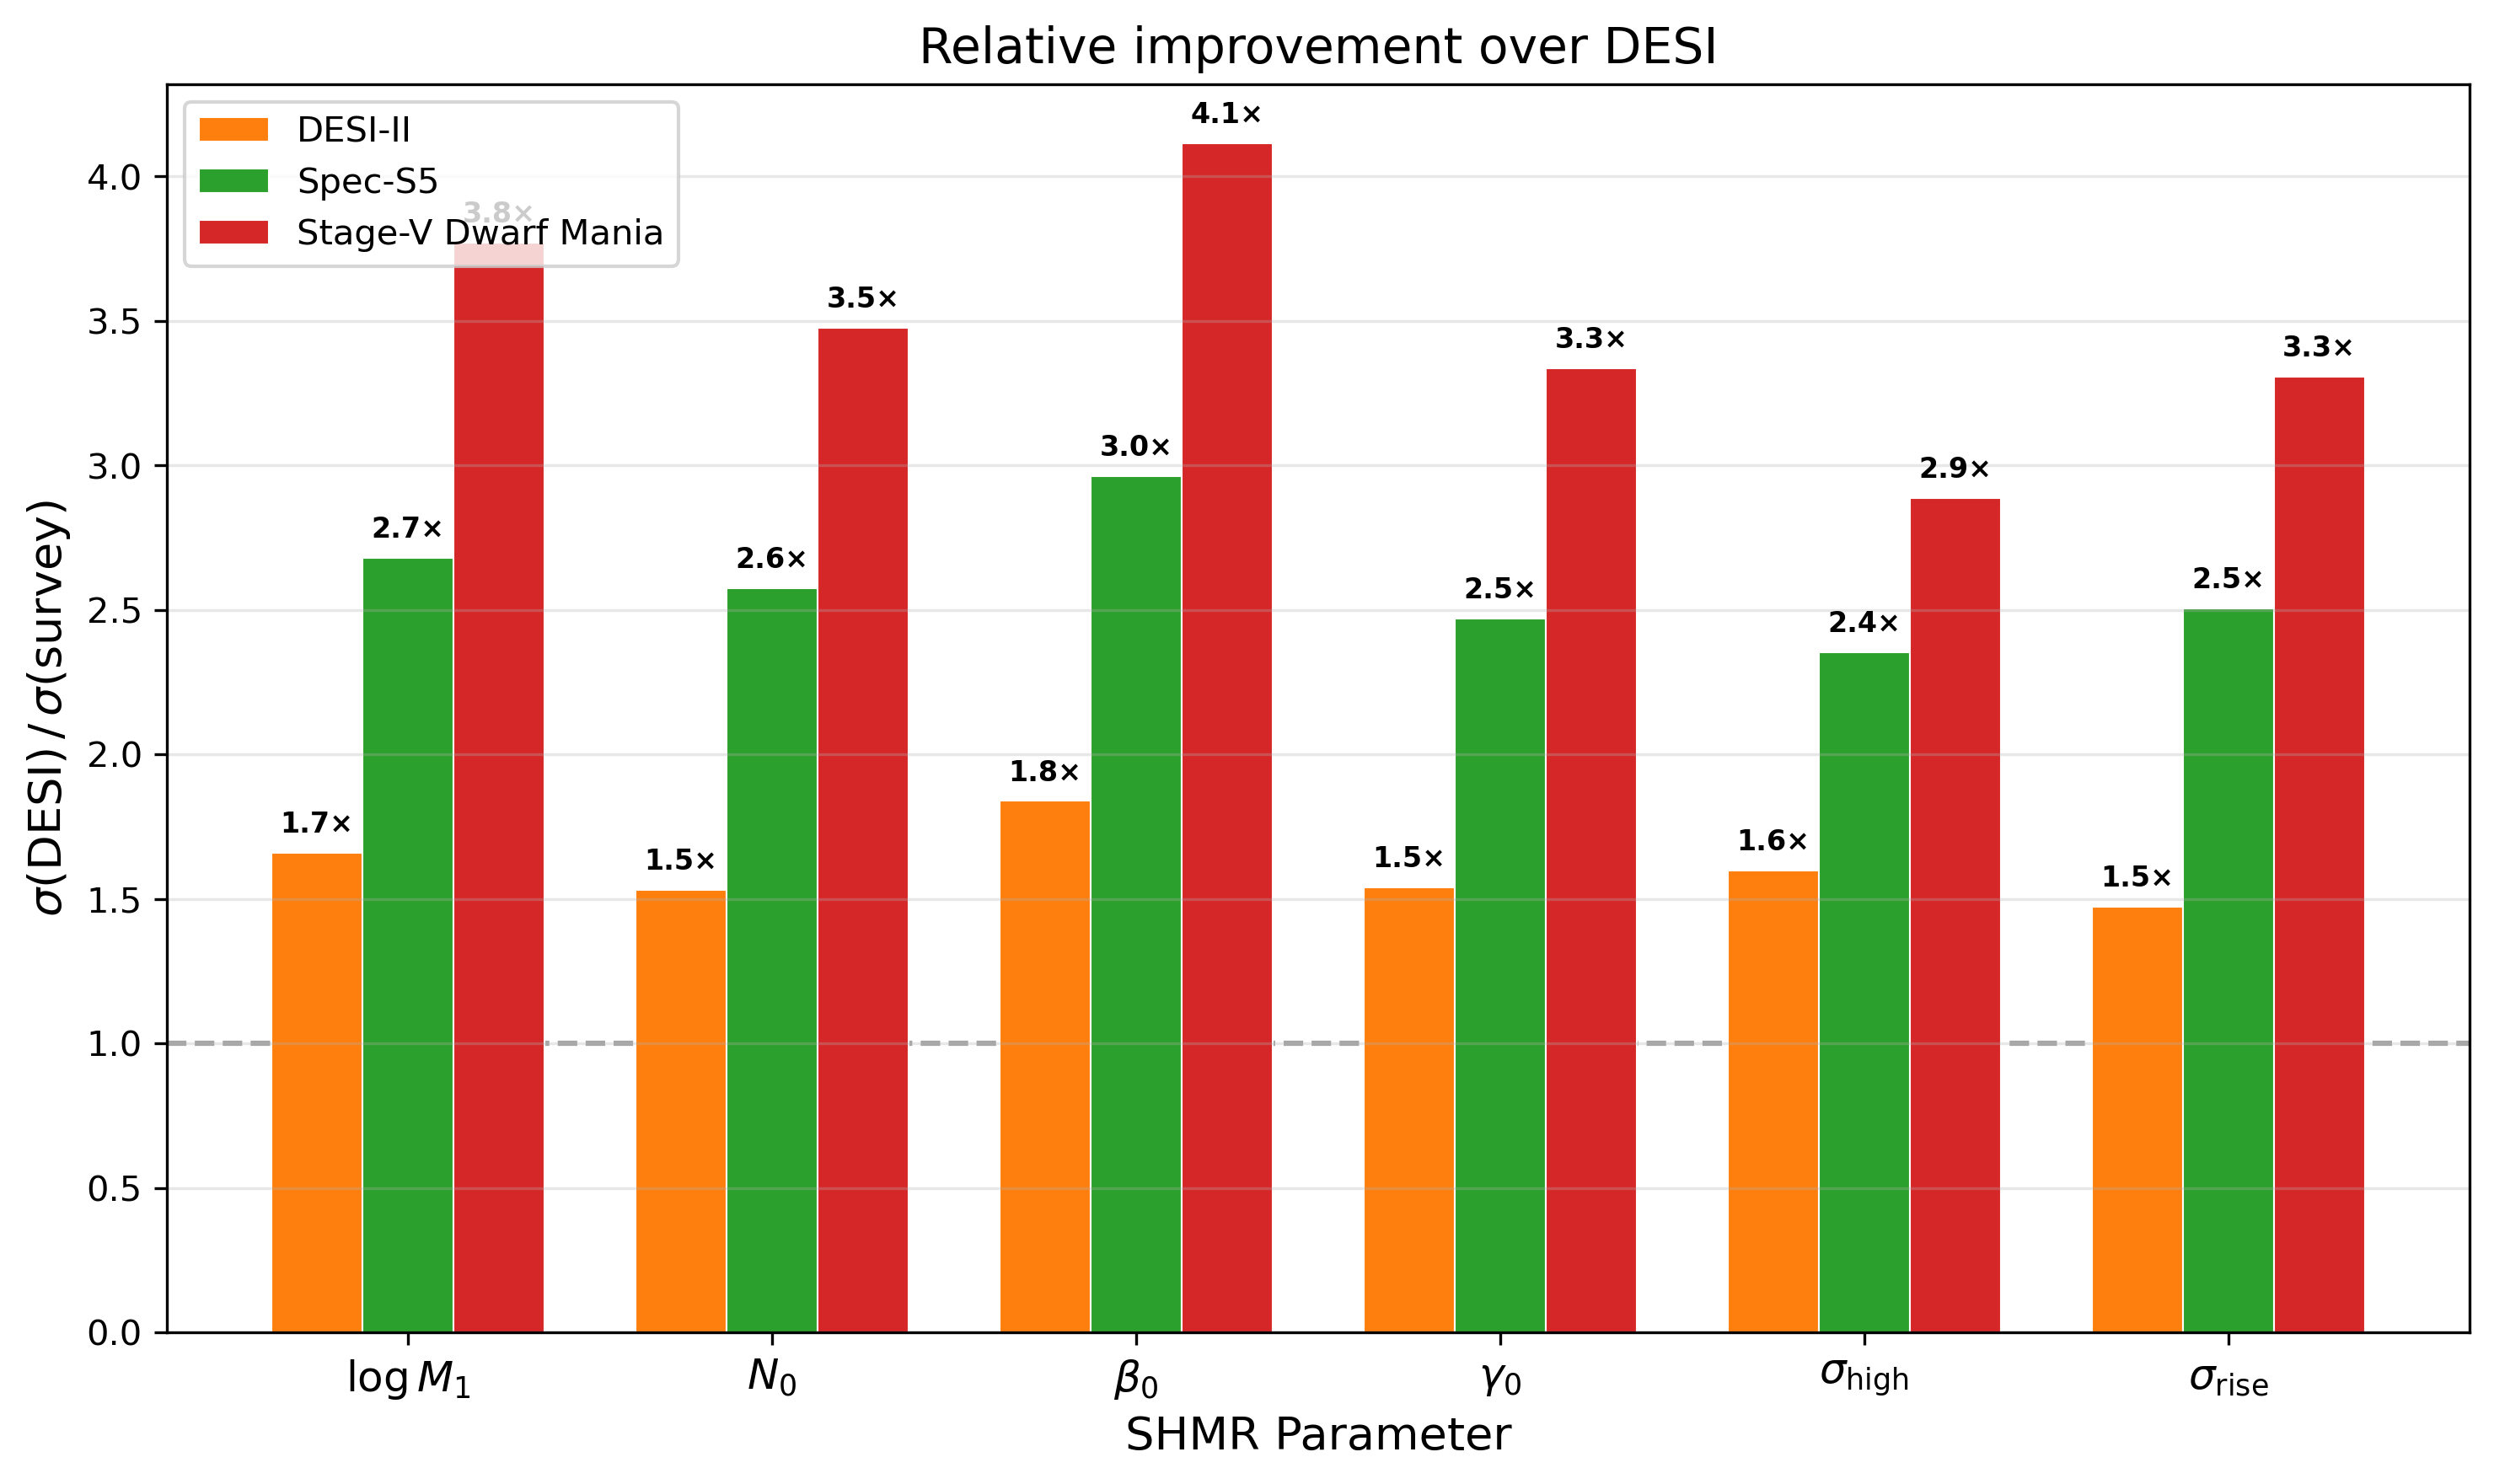
\includegraphics[width=0.85\textwidth]{figures/fullrange_relative_improvement.png}
\caption{Improvement factor over DESI for the full stellar mass range.
The gains are more uniform across all six parameters compared to the
dwarf-only case, reflecting the complementary information from
high-mass and low-mass bins. Stage-V achieves $2.9$--$4.1\times$
improvement; Spec-S5 achieves $2.4$--$3.0\times$.}
\label{fig:fullrange_improvement}
\end{figure}


%% ================================================================
\section{Technical Details}
\label{sec:technical}

\subsection{SHMR Parameterization}

The mean SHMR follows the Moster et al.\ (2013) double power-law:
\begin{equation}
\frac{\Mstar}{\Mh} = \frac{2\,N(z)}
    {\left(\Mh / M_1(z)\right)^{-\beta(z)} +
     \left(\Mh / M_1(z)\right)^{\gamma(z)}},
\label{eq:shmr}
\end{equation}
where each shape parameter evolves linearly in the variable
$\zeta \equiv z/(1+z)$:
\begin{equation}
X(z) = X_0 + \nu_X \cdot \zeta.
\end{equation}

Fiducial values are from Moster et al.\ (2013) Table~1:
$\log M_{1,0} = 11.59$, $N_0 = 0.0351$, $\beta_0 = 1.376$,
$\gamma_0 = 0.608$.
The inverse relation $\Mh(\Mstar)$ is obtained via
\texttt{scipy.optimize.brentq} root-finding, exploiting the
monotonicity of the SHMR.

\subsubsection{Mass-Dependent Scatter}

At fixed halo mass, the stellar mass is log-normally distributed with
scatter following Cao \& Tinker (2020):
\begin{equation}
\sigma(\Mh) = \sigma_\mathrm{high} + \sigma_\mathrm{rise}
    \left[1 - \tanh\!\left(\frac{\log\Mh - \log\Mh^\mathrm{break}}
    {\delta}\right)\right],
\label{eq:scatter}
\end{equation}
with fiducial values $\sigma_\mathrm{high} = 0.18\,\mathrm{dex}$,
$\sigma_\mathrm{rise} = 0.10\,\mathrm{dex}$,
$\log\Mh^\mathrm{break} = 12.0$, $\delta = 0.4\,\mathrm{dex}$.
The asymptotic scatter is $0.18\,\mathrm{dex}$ at high $\Mh$
(cluster-scale halos) and $0.38\,\mathrm{dex}$ at low $\Mh$ (dwarf
halos).
Only $\sigma_\mathrm{high}$ and $\sigma_\mathrm{rise}$ are varied in
the Fisher matrix; the transition mass and width are held fixed.


\subsection{Halo Occupation Distribution}

The continuous SHMR with scatter is converted into a halo occupation
distribution (HOD) for each stellar mass bin $[\log\Mstar^\mathrm{lo},
\log\Mstar^\mathrm{hi}]$:
\begin{equation}
\langle N_\mathrm{cen}(\Mh)\rangle = \frac{1}{2}
    \left[\mathrm{erf}(x_\mathrm{hi}) -
          \mathrm{erf}(x_\mathrm{lo})\right],
\quad
x = \frac{\log\Mstar^\mathrm{edge} -
          \langle\log\Mstar\rangle(\Mh)}
         {\sqrt{2}\,\seff(\Mh)},
\label{eq:ncen}
\end{equation}
where $\seff(\Mh) = \sqrt{\sSHMR^2(\Mh) + \sobs^2}$ is the effective
scatter incorporating stellar mass measurement uncertainty.
For spectroscopic surveys, we adopt $\sobs = 0.1\,\mathrm{dex}$.

Satellites follow Leauthaud et al.\ (2012):
\begin{equation}
\langle N_\mathrm{sat}(\Mh)\rangle =
    \langle N_\mathrm{cen}^\mathrm{thresh}\rangle \cdot
    \left(\frac{\Mh}{M_{1,\mathrm{sat}}}\right)^{\alpha_\mathrm{sat}},
\end{equation}
with $M_{1,\mathrm{sat}} = 17\,M_\mathrm{min}$ and
$\alpha_\mathrm{sat} = 1.0$.
Satellite parameters are fixed (not varied in the Fisher matrix); this
is acceptable for relative survey comparisons.


\subsection{Observable Predictions}

\subsubsection{Galaxy--Galaxy Lensing}

The bin-averaged excess surface mass density is:
\begin{equation}
\DS(R\,|\,\mathrm{bin}, z) = \frac{
    \int d\Mh \frac{dn}{d\Mh}\,N_\mathrm{tot}(\Mh)
    \left[\DS_\mathrm{NFW}(R, \Mh, z) +
          b_h(\Mh, z)\,\DS_\mathrm{mm}(R, z)\right]
}{n_\mathrm{gal}},
\label{eq:ds}
\end{equation}
where $dn/d\Mh$ is the Tinker et al.\ (2008) halo mass function,
$\DS_\mathrm{NFW}$ uses the Wright \& Brainerd (2000) analytic
expression with Diemer \& Kravtsov (2019) concentrations and the
\texttt{200m} mass definition, and $b_h$ is the Tinker et al.\ (2010)
linear halo bias.
The 2-halo matter term $\DS_\mathrm{mm}(R, z)$ is computed from the
nonlinear matter correlation function via line-of-sight projection
(truncated at $\pi_\mathrm{max} = 100\,\mathrm{Mpc}$) and cached per
redshift.

All integrals use the trapezoidal rule on a log-spaced grid of 200
halo masses spanning $\log\Mh \in [10.0, 15.5]$.
Colossus NFW profiles work in comoving $\mathrm{kpc}/h$; the
conversion to physical $\Msun/\mathrm{Mpc}^2$ is:
\begin{equation}
\DS_\mathrm{phys} = \DS_\mathrm{colossus} \times h \times 10^6
    \times (1+z)^2.
\end{equation}


\subsubsection{Effective Bias}

\begin{equation}
\beff(\mathrm{bin}, z) = \frac{
    \int d\Mh \frac{dn}{d\Mh}\,N_\mathrm{tot}(\Mh)\,b_h(\Mh, z)
}{\ngal}.
\end{equation}


\subsubsection{Stellar Mass Function}

\begin{equation}
\Phi(\mathrm{bin}, z) = \ngal = \int d\Mh \frac{dn}{d\Mh}\,
    N_\mathrm{tot}(\Mh) \quad [\mathrm{Mpc}^{-3}].
\end{equation}


\subsection{Covariance Models}

\subsubsection{Lensing Covariance}

The lensing covariance is diagonal (no off-diagonal radial bin
correlations) and shape-noise dominated:
\begin{equation}
\mathrm{Var}(\DS_i) = \frac{\sigma_e^2 \,\Sigma_\mathrm{crit,eff}^2}
    {N_\mathrm{lens} \cdot n_\mathrm{source,eff} \cdot A_{\mathrm{ann},i}}
    + \left(f_\mathrm{sys}\,\DS_\mathrm{fid}\right)^2,
\label{eq:var_ds}
\end{equation}
where $A_{\mathrm{ann},i} = \pi(R_\mathrm{hi}^2 - R_\mathrm{lo}^2)$
is the annulus area in physical $\mathrm{Mpc}^2$,
$\Sigma_\mathrm{crit,eff}$ is the effective critical surface mass
density averaged over a Smail-type source redshift distribution
$n(z_s) \propto z_s^2\,\exp[-(z_s/z_0)^{1.5}]$, and
$n_\mathrm{source,eff}$ is the effective source density behind the
lens redshift.
The systematic floor $f_\mathrm{sys} = 0.05$ accounts for baryonic
effects, miscentering, and photometric calibration.


\subsubsection{Clustering Covariance}

The effective bias variance includes cosmic variance and shot noise
via the FKP-weighted effective volume:
\begin{equation}
\mathrm{Var}(\beff) = \frac{\beff^2}
    {\ngal \cdot V_\mathrm{eff}},
\quad
V_\mathrm{eff} = V_\mathrm{survey} \cdot
    \left[\frac{nPb^2}{1 + nPb^2}\right]^2,
\end{equation}
where $P$ is evaluated at $k = 0.1\,h/\mathrm{Mpc}$.


\subsubsection{SMF Covariance}

The SMF covariance includes Poisson noise and cosmic variance:
\begin{equation}
\mathrm{Var}(\Phi) = \frac{\Phi}{V_\mathrm{survey}}
    + \beff^2\,\sigma_m^2(V, z)\,\Phi^2,
\label{eq:var_smf}
\end{equation}
where $\sigma_m^2(V, z)$ is the matter variance on the survey scale,
computed from the colossus matter power spectrum with a top-hat window
function of volume $V$.
In the Poisson-dominated regime (small $V$ or rare populations),
$\sigma(\Phi)/\Phi \approx 1/\sqrt{N}$.
In the cosmic-variance-dominated regime (large $V$, abundant
populations), $\sigma(\Phi)/\Phi \approx \beff\,\sigma_m$, which
sets an irreducible floor that does not decrease with more galaxies.


\subsection{Fisher Matrix Assembly}

\subsubsection{Parameter Selection}

The varied parameter set depends on the forecast configuration:
\begin{itemize}
    \item \textbf{Dwarf-only:} $N_0$, $\beta_0$,
    $\sigma_\mathrm{high}$, $\sigma_\mathrm{rise}$ (4 SHMR
    parameters), plus shear calibration $m$ and source photo-$z$ bias
    $\delta z_s$ (2 nuisance, with Gaussian priors $\sigma_m = 0.02$
    and $\sigma_{\delta z} = 0.03$). The high-mass parameters
    $\gamma_0$ and $\log M_{1,0}$ are fixed because dwarf halos
    ($\Mh \ll M_1 \sim 10^{11.6}\,\Msun$) are insensitive to them.

    \item \textbf{Full-range:} $\log M_{1,0}$, $N_0$, $\beta_0$,
    $\gamma_0$, $\sigma_\mathrm{high}$, $\sigma_\mathrm{rise}$
    (6 SHMR parameters), plus the same 2 nuisance parameters.

    \item \textbf{No $z$-evolution:} Since all surveys have
    $z_\mathrm{max} \le 0.3$, the evolution parameters
    ($\nu_{M_1}$, $\nu_N$, $\nu_\beta$, $\nu_\gamma$) are not varied.
\end{itemize}


\subsubsection{Numerical Derivatives}

Derivatives of observables with respect to SHMR parameters are
computed via central finite differences:
\begin{equation}
\frac{\partial f}{\partial \theta_i} \approx
    \frac{f(\theta_i + \delta) - f(\theta_i - \delta)}{2\delta},
\quad
\delta = 0.01 \times |\theta_i|.
\end{equation}
For parameters near zero ($|\theta_i| < 10^{-10}$), an absolute step
of $0.01$ is used.
Nuisance parameter derivatives are analytic.


\subsubsection{Fisher Accumulation}

For each (redshift bin, stellar mass bin), the Fisher matrix receives
three additive contributions:
\begin{equation}
F = \sum_\mathrm{bins} \left[
    J_\DS^\top\,C_\DS^{-1}\,J_\DS
    + \frac{J_b\,J_b^\top}{\mathrm{Var}(b_\mathrm{eff})}
    + \frac{J_\Phi\,J_\Phi^\top}{\mathrm{Var}(\Phi)}
\right],
\label{eq:fisher}
\end{equation}
where $J_\DS$, $J_b$, $J_\Phi$ are the Jacobian matrices of the
lensing, bias, and SMF observables, and $C_\DS$ is the diagonal
lensing covariance.
Gaussian priors on nuisance parameters are added to the Fisher
diagonal after accumulation.


\subsubsection{Post-Processing}

Marginalized 1$\sigma$ errors:
$\sigma(\theta_i) = \sqrt{(F^{-1})_{ii}}$.
Fisher ellipses for parameter pairs $(i, j)$ are computed from the
$2\times2$ sub-covariance of $F^{-1}$ via eigendecomposition.
The $1\sigma$ ellipse corresponds to
$\Delta\chi^2 = 2.30$ (68.3\% CL for 2 parameters), and the
$2\sigma$ ellipse to $\Delta\chi^2 = 6.18$ (95.4\% CL).
The condition number of $F$ is checked; values $>10^{10}$ trigger a
warning.


\subsection{Stellar Mass Measurement Uncertainty}

Observed stellar masses carry a statistical uncertainty
$\sobs \approx 0.1\,\mathrm{dex}$ for spectroscopic surveys.
This is incorporated exactly by replacing the intrinsic scatter
$\sSHMR(\Mh)$ with the effective scatter
$\seff(\Mh) = \sqrt{\sSHMR^2(\Mh) + \sobs^2}$ in the HOD
computation (Eq.~\ref{eq:ncen}).
This is the exact convolution of two Gaussians in log-space; no
numerical integration is needed.

The impact is largest at high halo masses where $\sSHMR$ is smallest
($0.18\,\mathrm{dex}$, giving $+15\%$ increase in effective scatter).
For dwarf galaxies ($\sSHMR \approx 0.38\,\mathrm{dex}$), the effect
is negligible ($+3\%$ in quadrature).


\subsection{Binning and Integration}

\begin{itemize}
    \item \textbf{Redshift bins:} edges from $z_\mathrm{min}$ to
    $z_\mathrm{max}$ in steps of $\Delta z = 0.2$; each bin evaluated
    at $z_\mathrm{mid}$.
    For the dwarf surveys ($z_\mathrm{max} \le 0.3$), this yields a
    single redshift bin.
    \item \textbf{Stellar mass bins:} from $\log\Mstar_\mathrm{min}$
    to $\log\Mstar_\mathrm{max}$ in steps of $0.5\,\mathrm{dex}$.
    \item \textbf{Radial bins for lensing:} 30 log-spaced bins from
    $R_\mathrm{min} = 0.01$ to $R_\mathrm{max} = 10\,\mathrm{Mpc}$.
    \item \textbf{Halo mass grid:} 200 log-spaced points from
    $\log\Mh = 10.0$ to $15.5$.
\end{itemize}


\subsection{Cosmology}

All calculations adopt Planck 2018 cosmology (Planck Collaboration
2020) via \texttt{colossus}:
$h = 0.6736$, $\Omega_m = 0.3153$, $\Omega_b = 0.0493$,
$\sigma_8 = 0.8111$, $n_s = 0.9649$.


%% ================================================================
\section{Key Assumptions and Limitations}
\label{sec:limitations}

\begin{enumerate}
    \item \textbf{NFW + linear 2-halo term.}
    The 1-halo--2-halo transition region ($R \sim 1$--$3\,\mathrm{Mpc}$)
    is not explicitly modeled; the two terms are summed directly. This
    double-counts matter near the virial radius but has negligible
    impact on the Fisher matrix, which depends on parameter derivatives
    rather than absolute signal levels.

    \item \textbf{Diagonal lensing covariance.}
    Off-diagonal correlations between radial bins from large-scale
    structure are not included, leading to mildly optimistic
    constraints.

    \item \textbf{Clustering compressed to $\beff$ + SMF.}
    The full $w_p(r_p)$ information content is compressed to a single
    bias value per bin, discarding scale-dependent clustering
    information.

    \item \textbf{Fixed satellite prescription.}
    Satellite parameters ($\alpha_\mathrm{sat}$, $M_1/M_\mathrm{min}$)
    are not varied; absolute error bars should be interpreted with
    this caveat.

    \item \textbf{No scatter redshift evolution.}
    $\sigma(\Mh)$ is assumed constant with $z$, consistent with
    Behroozi et al.\ (2019).

    \item \textbf{No covariance between stellar mass bins.}
    Each $(z, \Mstar)$ bin contributes independently. Overlapping halo
    populations create inter-bin correlations that are not modeled.

    \item \textbf{Unbiased stellar mass estimator.}
    Only statistical scatter ($\sobs$) is included; systematic biases
    in stellar mass estimation are not modeled.
\end{enumerate}


%% ================================================================
\section*{References}
\label{sec:references}

\begin{itemize}
\item Behroozi, P., et al., 2019, MNRAS, 488, 3143
\item Cao, J., \& Tinker, J.~L., 2020, MNRAS, 498, 5080
\item Diemer, B., 2019, ApJS, 239, 35
\item Diemer, B., 2023, ApJ, 947, 59
\item Eisenstein, D.~J., \& Hu, W., 1998, ApJ, 496, 605
\item Leauthaud, A., et al., 2012, ApJ, 744, 159
\item Moster, B.~P., Naab, T., \& White, S.~D.~M., 2013, MNRAS, 428, 3121
\item Oguri, M., \& Takada, M., 2011, PRD, 83, 023008
\item Planck Collaboration, 2020, A\&A, 641, A6
\item Smith, R.~E., et al., 2003, MNRAS, 341, 1311
\item Tegmark, M., Taylor, A.~N., \& Heavens, A.~F., 1997, ApJ, 480, 22
\item Tinker, J.~L., et al., 2008, ApJ, 688, 709
\item Tinker, J.~L., et al., 2010, ApJ, 724, 878
\item Wright, C.~O., \& Brainerd, T.~G., 2000, ApJ, 534, 34
\end{itemize}


\end{document}
